\documentclass[11pt]{article}
\usepackage{amsmath}

\usepackage{algorithm}
%\usepackage{algpseudocode}}

\usepackage[framemethod=TikZ]{mdframed}
\mdfdefinestyle{MyFrame}{%
    linecolor=blue,
    outerlinewidth=1pt,
    roundcorner=10pt,
    innertopmargin=\baselineskip,
    innerbottommargin=\baselineskip,
    innerrightmargin=20pt,
    innerleftmargin=20pt,
    backgroundcolor=white}

\makeatletter
\def\BState{\State\hskip-\ALG@thistlm}
\makeatother
\usepackage{hyperref}
\hypersetup{colorlinks=true,linkcolor=blue,urlcolor=blue}

\usepackage{amsfonts}
\usepackage[utf8]{inputenc}
\usepackage[english]{babel}
\usepackage{amsthm}
\usepackage{bbm}
\usepackage{xcolor}
%\usepackage[dvipsnames]{xcolor}
\usepackage{longtable}
\usepackage{booktabs, caption, makecell}
\renewcommand\theadfont{\bfseries}
\usepackage{threeparttable}
\DeclareMathAlphabet{\mathpzc}{OT1}{pzc}{f}{it}
\DeclareMathOperator*{\argmax}{argmax}
\usepackage{appendix}
\newtheorem{innercustomthm}{Theorem}
\theoremstyle{plain}
\usepackage{graphicx}
\usepackage{wrapfig}
\usepackage{parskip}% http://ctan.org/pkg/parskip 
\usepackage{adjustbox}
\usepackage{lipsum}
\usepackage{tabularx}
\usepackage{listings}
\newtheorem{exercise}{Exercise}
\newtheorem{proposition}{Proposition}[section]
\newtheorem{assumption}{Assumption}[section]
\newtheorem{theorem}{Theorem}[section]
\newtheorem{corollary}{Corollary}[proposition]
\newtheorem{lemma}[theorem]{Lemma}
\newtheorem{myassum}{Assumption}
\newtheorem{definition}{Definition}[section]
\newenvironment{customthm}[1]
{\renewcommand\theinnercustomthm{#1}\innercustomthm}
{\endinnercustomthm}


\usepackage{biblatex}
%\addbibresource{refs.bib}


%\usepackage[toc,page]{appendix}
%\usepackage{import}

\usepackage{geometry}
\usepackage{marginnote}

\title{\textbf{Keeping TABS}\\
\small{A Canonical-Arbitration Algorithm for Modified-GHOST PoW Blockchain Protocols}}

%% NOMENCLATURE: "Keeping TABS" is a play on words.
%% The phrase is an english idiom used to describe a state of watchfulness or
%% reactive observation, as in: I must keep tabs on my bank account to ensure that
%% I understand my finanical status and to prevent miscalculations.
%% In the use of the conjugated form of the verb "to keep," we find also a
%% reference to the action of preservation, or a suggested state of permanence.
%% With this, the play on words ultimately suggests that observation of some
%% state is associated with the persistence of the state itself.
%% This is an effective and accurate illustration of both the means and ends of
%% this project.
%% In spite of the cost of explaining a joke, we hope this provides clarity for
%% non-native English readers and harmless interpretive confirmation otherwise.

\author{Isaac Ardis\
\and Daniel Aronoff\\\small{MIT Economics}\\\small{MIT Media Lab}}

\begin{document}

%% %%%%%%%%%%%%%%%%%%%%%%%%%%%%%%%%%%%%%%%%%%%%%%%%%%%%%%%%%%%%%%%%%%%%%%%%%%%%%%%%%%%%%%%%%%%%%%%%%%%%%%%%%%

\maketitle
\begin{abstract}

Canonical-arbitration algorithms are used to build consensus in decentralized
state machines.
The consensus characteristics of mutually implemented canonical-arbitration
algorithms enables a race between block authors and thereby facilitate
the trust-minimized security characteristics of the blockchain state.
%In Proof-of-Work (PoW) block emission systems, canonical-arbitration
%algorithms are often co-dependent with dynamic emission parameters (eg.
%Difficulty).

We consider a proposed modification to the "Modified GHOST" algorithm in use on
Ethereum.\footnote{\url{https://ethereum.org/en/whitepaper/#modified-ghost-implementation}}
This proposal introduces two novel features: a capacity for segment-specific
transactions, and a positive scalar value representing a general measurement of
active capital.
From these features we propose a novel condition program situated in an assumed
incumbent canonical-arbitration algorithm.

Our proposed design is an augmentation of an existing and widely implemented consensus program.
As such, it assumes and depends on the existence of other (canonical-arbitration)
algorithmic conditions.
We inherit and generally preserve as invariants the characteristics of the incumbent canonical-arbitration algorithm.

We claim and attempt to demonstrate that the proposed algorithmic condition
program raises the incumbent consensus decidability rate.
We show that this increased decidability rate improves chain state finality
characteristics and reduces network energy waste by 50\%.
Further, we show that the cost to an adversary in a double-spend attack scenario rises.
We detail any associated additional risk to the network, which we show to
be practically nominal.
We note that implementation of this design is feasible for Ethereum's
primary client \textit{go-ethereum} (\texttt{geth}) and probably feasible for
most existing PoW clients.

\end{abstract}

\pagebreak

%% %%%%%%%%%%%%%%%%%%%%%%%%%%%%%%%%%%%%%%%%%%%%%%%%%%%%%%%%%%%%%%%%%%%%%%%%%%%%%%%%%%%%%%%%%%%%%%%%%%%%%%%%%%

\section{\normalsize{Model Definitions}}

\begin{table}[H]
\caption{List of Model Definitions\label{table: model-definitions}}
\centering
\small{
\begin{tabular}{|p{5cm}|p{9cm}|}

\hline
\multicolumn{2}{| c |}{Model Elements} \\
\hline
\hline
$t$ & Unit of time. Standard unit: seconds. \\~\\

$\lambda$ & Network mean block time; the average number of seconds between
block timestamps. \\~\\

$\eta$ & Network block-message latency (measurable or assumed) between two
nodes. The time elapsed between the transmission of a message containing block
information and its reception. \\~\\

$B_i$ & A block with number $i$. \\~\\
$H_i$ & A block header with number $i$. \\~\\

$H_d$ & Block (and header) annotated difficulty \\~\\
$H_k$ & Block (and header) annotated $\mathrm{TABS}$ value \\~\\

$TAB(B)$ & A scalar value representing aggregated account balances for a given
block $B$. "TAB" stands for Total Active Balance. \\~\\
$TABS(B_i,B_{\mathrm{i-1}})$ & A scalar value derived from the $TAB$ value of
block $B_i$ and recursively its parent $B_{i-1}$. This value is annotated in a
block's header. "S" stands for \textit{synthetic} or \textit{synthesis}. \\~\\

$\sigma[a]$ & Global account state $\sigma$ at address $a$ \\~\\

$T$ & A transaction \\~\\

$T_a$ & A proposed transaction field: Ancestor Hash \\~\\

$\delta(T_a)$ & The depth (magnitude of ancestry) of a block cited by some
transaction as $T_a$ \\~\\

$\tau$ & A network-level aggregate over time or segment (assume: average) of
Ancestor Hash depth $\delta$ values. Transactions \textit{not} asserting an
Ancestor Hash value can be defined as having $\delta$ = $H_i$.
Smaller values represent a greater dependence on blocks nearer a common
(consensus) chain head (a greater degree of transaction/segment exclusivity),
while larger values signal less exclusive transactional assertion on chain
state dependence.
\\~\\

$\mathrm{CS}$ & Canon Score. A scalar value representing canon preference
weight of a single block. Comparable to Difficulty. \\~\\

$\mathrm{TCS}$ & Total Canon Score. A scalar value representing protocol
canonical preference. Derivation of this value for any block relies on the
antecedent calculation of that of its parent. Comparable to Total Difficulty.
\\~\\

\hline
\end{tabular}
}
\end{table}

%% %%%%%%%%%%%%%%%%%%%%%%%%%%%%%%%%%%%%%%%%%%%%%%%%%%%%%%%%%%%%%%%%%%%%%%%%%%%%%%%%%%%%%%%%%%%%%%%%%%%%%%%%%%

\section{\normalsize{Glossary}}

\begin{table}[H]
\caption{Definitions of Common Terms\label{table: common-terms}}
\centering
\small{
\begin{tabular}{|p{5cm}|p{9cm}|}

\hline
\multicolumn{2}{| c |}{Glossary} \\
\hline
\hline

Ancestor Hash &
A proposed transaction field whose value references
a block by hash, specifying the existence of that block in the transaction's
chain segment as a condition of the transaction's validity.
Proposed. Optional.
Synonyms: Segment ID, HFC (Header Field Context) Hash.
Related: Chain ID.
\\~\\

Canonical-Arbitration Algorithm &
A program of
comparative conditions resulting in the selection of one prioritized segment from any two segments.
In context, the prioritized segment is used as the basis
for determining a canonical chain state, and, as such, for focusing mining
effort (via establishing a \textit{parent}.
Synonyms: Canonical-Preference
Algorithm.
Related: GHOST, Modified GHOST, Inclusive Protocol, Nakamoto Protocol.
\\~\\
%% $Canonical-Arbitration Algorithm & A program of comparative
%% conditions resulting in the selection of one prioritized segment from any two
%% segments. In context, the prioritized segment is used as the basis for
%% determining a canonical chain state, and, as such, for focusing mining effort
%% (via establishing a \textit{parent}. Synonyms: Canonical-Preference 
%% Algorithm.
%% Related: GHOST, Modified GHOST, Inclusive Protocol, Nakamoto Protocol. \\~\\

Segment-Agnostic (Transaction) &
A property on a transaction such that the transaction can be applied to one or more chain histories.
Related: Segment-Specific.
\\~\\

Segment-Specific (Transaction) &
A property on a transaction such that the transaction can be applied on a subset of available chain histories.
Synonyms: Segment-Exclusive, Chain Context Constrained.
Related: Segment-Agnostic.
\\~\\

Chain State Finality &
The permanence of chain state (or series of
states).
PoW blockchain states have characteristically `soft` finality
characteristics.
PoW finality expectations increase as relative state
increases; newer states are more vulnerable to change than older states.
\\~\\

Block Emissions &
The (rate of) production of blocks. Blocks are
metadata associated with chain state modification sequences.
\\~\\

\hline
\end{tabular}
}
\end{table}

%% %%%%%%%%%%%%%%%%%%%%%%%%%%%%%%%%%%%%%%%%%%%%%%%%%%%%%%%%%%%%%%%%%%%%%%%%%%%%%%%%%%%%%%%%%%%%%%%%%%%%%%%%%%

\section{\normalsize{Scenarios}}

\begin{table}[H]
\caption{Outlines of Referenced Chain State Scenarios \label{table: chainstate-scenarios}}
\centering
\small{
\begin{tabular}{|p{5cm}|p{9cm}|}

\hline
\multicolumn{2}{| c |}{Scenarios} \\
\hline
\hline

Finality Fraud & A premeditated fraud scheme exploiting a victim's
assumption of chain state which is later invalidated by the attacker.
The exemplary scenario defined and reused throughout this paper assumes a single
entity as a victim and a single censored transaction.
In most contexts, these assumed parameters could be modified to use a plural set of victim entities
and/or a plural set of censored transactions while still being considered Finality Fraud.
\\~\\

Finality Terrorism & Generally schematically equivalent to Finality
Fraud; the difference is in the attacker's motive and an intentionally large number of victims.
The exemplary scenario defined and reused throughout this paper
assumes all users of a blockchain as victims and the censorship of all transactions.
These parameters are extremes.
In most contexts, these assumed parameters could be modified while still being considered Finality Terrorism.
\\~\\

\hline
\end{tabular}
}
\end{table}

%% \pagebreak
%% \section{\normalsize{Proposal Context}}

%% \subsection{\small{Related Works}}\label{sec: S1.-1}

%% - Eyal and Sirer: Thwarting Selfish Mining with a Coin-Toss \\
%% - Freshness-Preferred. (Cited for augmentative structure of proposal; not
%% for risk costs or security characteristics.)

%% \subsection{\small{Inherited Assumptions}}\label{sec: S1.0}

%% We assume in all non-general cases theoretical inheritance from the Ethereum
%% (ETH) protocol, which differs only trivially in this context from the 
% Ethereum
%% Classic (ETC) protocol.\footnote{https://github.com/ethereum/yellowpaper}

%% As noted in the Abstract, we take this context for granted as a necessary
%% assumption for the sake of argument.
%% However, we hypothesize, but do not attempt to show, the parameters and
%% validity of a more general case (eg. applicable for most PoW protocols).

%% We assume that all players in the presented theoretical games are
%% self-interested and infinitely greedy.

%% %%%%%%%%%%%%%%%%%%%%%%%%%%%%%%%%%%%%%%%%%%%%%%%%%%%%%%%%%%%%%%%%%%%%%%%%%%%%%%%%%%%%%%%%%%%%%%%%%%%%%%%%%%

\pagebreak
\section{\normalsize{Appendix: Ethereum Background}}

The parameters and logic of this paper's proposal take the existence of a
system equivalent with that of Ethereum's at the time of writing.
We strongly suggest that the Ethereum Yellow Paper\nolinebreak
\footnote{https://github.com/ethereum/yellowpaper/tree/fabef2531a8f8e772a4bf5be23191044d0ce3569}
be read and understood as a precondition for interpretation and evaluation
of the work of this project.
%should we state the 'Berlin' version? ISAAC: Done.
Important and referenced concepts of Ethereum's protocol are discussed in this 
section for the the informational value of redundancy.

\subsection{\small{Ethash}}\label{sec: S1.1}

Ethereum's Proof-of-Work protocol "Ethash" governs block emissions. Solutions
to a constantly varying guessing game require time to discover -- via trial and
error -- and are a notably required field in block headers. Authors of blocks
providing valid solutions to these puzzles are called miners; mining is the
process of searching for puzzle solutions. \\
\\
%should we define "block emissions" for the non-expert?
A very difficult puzzle (probably requiring many guesses) is expected to take 
more time to solve than an easier puzzle (requiring fewer guesses).

\subsection{\small{Difficulty}}\label{sec: S1.2}
Ethereum regulates its block emission rate using a header value called
$\mathrm{Difficulty}$ ($H_d$). This value is used by the Ethash protocol as a
parameter for puzzle solution validation. Generally speaking, the Difficulty
value for some block can be thought of as the number of wrong guesses
("hashes") expected before a valid puzzle solution for a child block is
found.\nolinebreak
\footnote{Formally, difficulty is governed by the relation of a fixed size
bit-field (called the 'nonce') in the domain of the block hash, into which a 
miner writes its guess, and a fixed size bit-field in the output range of the 
hash function, which takes on values induced by the miner's guess. The 
difficulty is measured by the number of required zero entries in the output  
bit-field, which defines the feasible output range.  The size of the set of 
guesses that map into the feasible range expands and contracts with the size of 
the feasible range. For a given rate of guesses per unit of time, the 
difficulty induces a cumulative distribution function of the probability of a 
solution being found by each point in time. From this an expected interval 
between timestamps can be derived.}
An adjustment algorithm governs the rise and fall of this value, accepting a 
block timestamp interval and parent difficulty as parameters;
this provides a feedback loop joining block emission rates (via sequential 
block timestamps and thus relative intervals) with puzzle difficulty.
Given a target block interval, difficulty can be adjusted dynamically, 
incrementally, such that the difficulty value will cause blocks to be authorable
at rates approaching the target rate.
In Ethereum the parameters are tuned to produce a median 9 seconds, or about 14
seconds on average.
Network block emission rates are typically modeled with a Poisson
distribution.\nolinebreak
\footnote{https://ethresear.ch/t/deep-dive-into-current-pow-difficulty-adjustmen
t-algorithm-and-a-possible-alternative/5267}\nolinebreak
\footnote{https://blog.ethereum.org/2015/09/14/on-slow-and-fast-block-times/}\nolinebreak
\footnote{https://en.wikipedia.org/wiki/Proof_of_work#Variants}\nolinebreak
\footnote{https://arxiv.org/pdf/1901.04620, Section III.A}

\textit{e.g.} Given a block difficulty $H_d$ = 63115 and a network target
emission interval of 13 seconds, we deduce that the modeled network average
hashrate is 63115 hashes / 13 seconds = 4855 hashes/second. A block generated
in 3 seconds should cause the difficulty to rise; a block generated in 30
seconds should cause it to fall; making the next block respectively harder or
easier (slower or faster) to author.

\subsection{\small{Canonical Arbitration}}\label{sec: S1.3}

The "Total Difficulty" value for any chain segment is the sum of the $H_d$ 
values of block headers in the segment.
The canonical-arbitration algorithm used today by Ethereum defines %instructs?
that preference is given with priority to any valid subtree having the greatest 
"Total Difficulty" value.
In the case of equivalent TD values, segments are preferred having lesser 
latest block numbers. (Shorter segments).
In the case of equivalent TD and block height (number) values, if a node acts 
on behalf of the block's registered author, that block is preferred.
If there is no authorship beneficiary interest (as in a non-mining node, or 
that of a non-winning miner), a figurative coin is tossed, per the protocol 
described by Eyal and Sirer.\nolinebreak
\footnote{http://www.cs.cornell.edu/~ie53/publications/btcProcFC.pdf}

\subsection{\small{Chain ID}}\label{sec: S1.4}

As specified by EIP155\nolinebreak
\footnote{https://eips.ethereum.org/EIPS/eip-155} a feature called
\textit{Chain ID} was introduced on the Ethereum network (ETH) at block
2675000, and on the Ethereum Classic network (ETC) at block 3000000.

This feature, generally considered, allows transactions to be made exclusive to
certain predefined segments, or entire chains, by validating a match between a
transaction-specified \textit{Chain ID} field value and that of a hardcoded
(constant) network protocol configuration.
The mechanism ascribes an arbitrary positive integer to a network configuration
and transactions use this value when signing a transaction intended for that
subset of chain state.
Transactions are not required to specify a \textit{Chain ID} value for
legacy-compatibility reasons.

This feature was introduced after "The DAO Fork" (at block 1920000) caused
Ethereum to become both Ethereum and Ethereum Classic, by the network's partial
rejection of an arbitrary chain state mutation.
Until the introduction of Chain ID, transactions after this hardfork had no way
of being exclusive to one of either of these two chains. Between blocks 1920000
and 2675000on ETH, transactions were ambiguously valid on either, or both.
Today, Chain ID transactions specifying Chain ID \texttt{1} are only eligible
on ETH, and those with Chain ID \texttt{61} are only eligible on ETC, per the
respective configurations eventually introduced on both networks with their
independent implementations of the EIP155 feature.


%% %%%%%%%%%%%%%%%%%%%%%%%%%%%%%%%%%%%%%%%%%%%%%%%%%%%%%%%%%%%%%%%%%%%%%%%%%%%%%%%%%%%%%%%%%%%%%%%%%%%%%%%%%%

\pagebreak
\section{\normalsize{Specifications}}

%Specifications for $TABS$?

In this section we describe the elements of the $TABS$ modification to the
"Modified GHOST" algorithm.

\subsection{\small{Transactions with Ancestor Hash}}\label{sec: S2.1}

Transactions are afforded an additional field $T_\mathrm{a}$ (\textit{Ancestor
Hash}) whose value either describes a block hash or is left undefined.

If filled, the existence of a block with a header matching this hash anywhere
in the ancestral, canonical chain (prior to the transaction's block) is a
condition of the transaction's validity.

Transactions of this type are considered segment-specific, although the degree
to which they are specific depends on which block is referenced by the hash is
provided.
Transactions referencing relatively older headers are less specific than those
referencing newer headers.

Transactions are not required to provide this value, but discretionary use is not 
necessary; the field \textit{could} be required.

We will show that the rate of this feature's use ($\tau$) will drive desirable
security characteristics of the proposed canonical-arbitration condition
program.

%Useful to have a graphic description here

\subsection{\small{TABS Validation}}\label{sec: S3.1}

TABS stands for Total Active Balance Synthesis.
%Maybe TABS should be defined in the Glossary
It is a positive scalar value intended to provide a representative measure of 
chain state capitalization.
It is denominated in Wei.
Its value will be used as a parameter in the proposed canonical-arbitration
condition.

\newcommand{\minTABS}{K_0}
\newcommand{\mynumerator}{y}
\newcommand{\diffadjustment}{x}

The validation of the TABS value of a block of header $H$ is asserted as
$\mathrm{TABS}(H)$, \\

where:
\begin{equation}
\mathrm{TABS}(H) \equiv \begin{cases}

\minTABS & \text{if} \quad H_{\mathrm{i}} = 0 \, \vert\vert \, P(H)_{H_k}
\text{is undefined} \\

\text{max}\!\left(\minTABS, {P(H)_{\mathrm{H}}}_{\mathrm{k}} +
\diffadjustment\times\mynumerator \right) & \text{otherwise} \\
\end{cases}
\end{equation}

where:
\begin{equation}
\minTABS \equiv 128\times 10^{18}
\end{equation}
\begin{equation}
\diffadjustment \equiv
\left\lfloor\frac{{P(H)_{\mathrm{H}}}_{\mathrm{k}}}{128}\right\rfloor
\end{equation}
\begin{equation}
y \equiv \begin{cases}
-1 & \text{if} \, $TAB(B)$ \, < \, $P(H)_{H_k}$ \\
0 & \text{if} \, $TAB(B)$ \, \equiv \, $P(H)_{H_k}$ \\
1 & \text{if} \, $TAB(B)$ \, > \, $P(H)_{H_k}$ \\
\end{cases}
\end{equation}

The \mathrm{TAB(B)} value of a block is defined as the sum of the miner balance
and all of the sender balances for transactions with an affirmative $T_a$
ancestor hash field:

\begin{equation}
TAB(B) \equiv L(B, B_c) \, + \, \sum_{T \in B_{\mathrm{txes}}}
L(B,T_{\mathrm{sender}})
\end{equation}

where:

\begin{equation}
L(B,s) \equiv P(B)_{\sigma[s]_{\mathrm{b}}} \quad \text{The account state
balance at parent block $P(B)$ of account $s$} \\
\end{equation}

The reader may note that the integer \texttt{128} appears shared between the
$x$ and $K_0$ components.
This is not of necessity, but of convenience and for simplicity of design.
Both values are tune-able constant parameters in the algorithm.
$K_0$ expresses a minimum value for $TABS$, while $x$ expresses an adjustment
ratio of the $TABS$ value between two parent-child related blocks.

%Here we deviate from the Eth yellow paper by omitting the 'freeze' parameter. 
I think this should be acknowledged in a footnote.

\subsection{\small{Canon Scoring}}\label{sec: S4}

Canonical-arbitration algorithms are assumed to compare two blocks and to
indicate decisively which one of the two ought to receive canonical status.
This section formally defines a value Canon Score \textit{CS}, which is used as
the \textit{initial condition} for a canonical-arbitration algorithm.
This condition, in both the pre-existing and proposed algorithms, may result in
a tie. If the condition is decisive (a winner is determined), subsequent
conditions are not evaluated.

If indecisive (the result is a tie), subsequent conditions are evaluated, each
potentially decisively, in program order.

For the sake of context, we write the assumed existing initial condition for
canonical-arbitration in our notation below.

The Canon Score value is defined as:

\begin{equation}
\mathrm{CS} \equiv H_d
\end{equation}

And derived from that a Total Canon Score for any segment as:

\begin{equation}
\mathrm{TCS} \equiv \sum_{H_\mathrm{i = 0}}^{\mathrm{i <= n}} H_d
\end{equation}

Respective to this assumed existing condition, we propose its modification as,

in the atomic case:

\begin{equation}
\mathrm{CS} \equiv H_d \times H_k
\end{equation}

and in the segment case:

\begin{equation}
\mathrm{TCS} \equiv \sum_{H_\mathrm{i = 0}}^{\mathrm{i <= n}} H_d \times H_k
\end{equation}

In both the pre-existing algorithm and the proposed algorithm, a candidate
block having a greater \textit{TCS} value than the other should be selected for
the exclusive canonical state.

%% %%%%%%%%%%%%%%%%%%%%%%%%%%%%%%%%%%%%%%%%%%%%%%%%%%%%%%%%%%%%%%%%%%%%%%%%%%%%%%%%%%%%%%%%%%%%%%%%%%%%%%%%%%

\pagebreak
\section{\normalsize{Visual Glossary}}

\begin{figure}[tph]
\centering
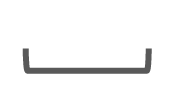
\includegraphics[width=0.2\textwidth]{vis_block.png}
\caption{A block}
\label{fig:block}
\end{figure}

\begin{figure}[tph]
\centering

\includegraphics[height=1cm]{vis_tx.png}
\caption{A transaction}
\label{fig:tx}
\end{figure}

\begin{figure}[tph]
\centering
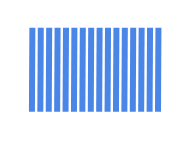
\includegraphics[width=0.2\textwidth]{vis_tx_set.png}
\caption{Several transactions}
\label{fig:txs}
\end{figure}

\begin{figure}[tph]
\centering
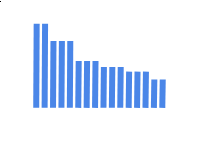
\includegraphics[width=0.2\textwidth]{vis_tx_set_sized.png}
\caption{Several transactions representing relative gas consumption}
\label{fig:txsgas}
\end{figure}

\begin{figure}[tph]
\centering
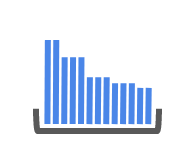
\includegraphics[width=0.2\textwidth]{vis_blocktxs.png}
\caption{Transactions in a block}
\label{fig:blocktxs}
\end{figure}

\begin{figure}[tph]
\centering

\includegraphics[width=1.0\textwidth]{vis_blocksegment.png}
\caption{A block segment (chain)}
\label{fig:blocksegment}
\end{figure}

\begin{figure}[tph]
\centering
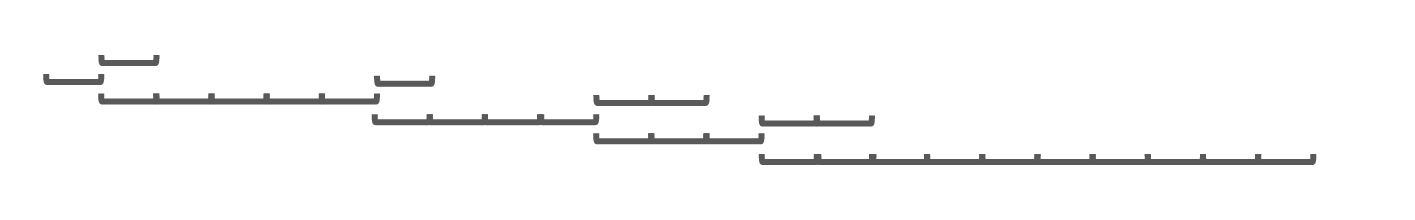
\includegraphics[width=1.0\textwidth]{vis_blocksegment_forking.png}
\caption{A block segment with forks}
\label{fig:blocksegment_forks}
\end{figure}

\begin{figure}[tph]
\centering
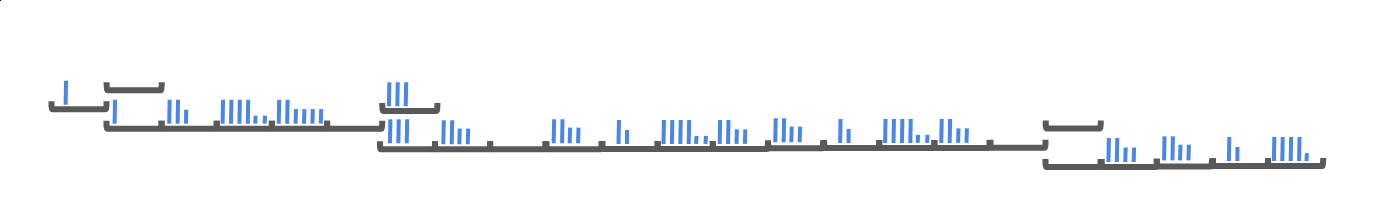
\includegraphics[width=1.0\textwidth]{vis_blocksegment_forking_txs_sparse.png}
\caption{A block segment with forks and sparse transactions}
\label{fig:blocksegment_forks_txs_sparse}
\end{figure}

\begin{figure}[tph]
\centering
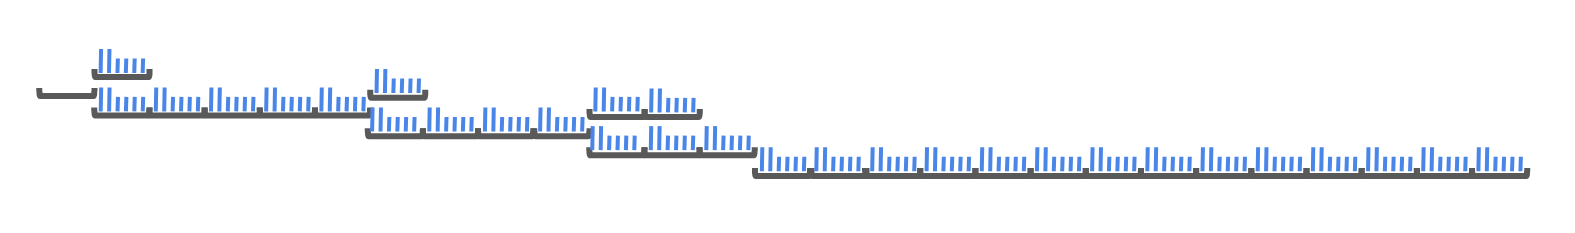
\includegraphics[width=1.0\textwidth]{vis_blocksegment_forking_txs_full.png}
\caption{A longer block segment with forks and full of transactions}
\label{fig:blocksegment_forks_txs_full}
\end{figure}


\begin{figure}[tph]
\centering
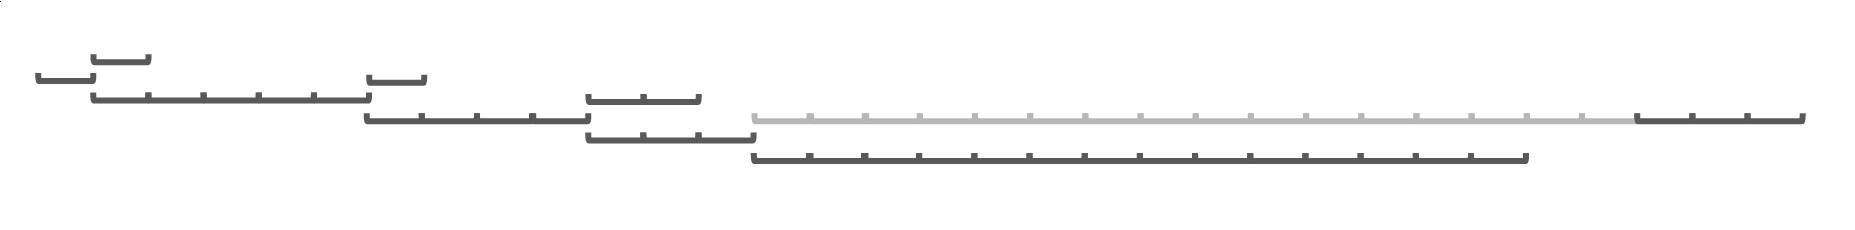
\includegraphics[width=1.0\textwidth]{vis_blocksegment_forking_reorg.png}
\caption{Block composition of a large reorg (eg. finality attack)}
\label{fig:blocksegment_forks_reorg}
\end{figure}

\begin{figure}[tph]
\centering
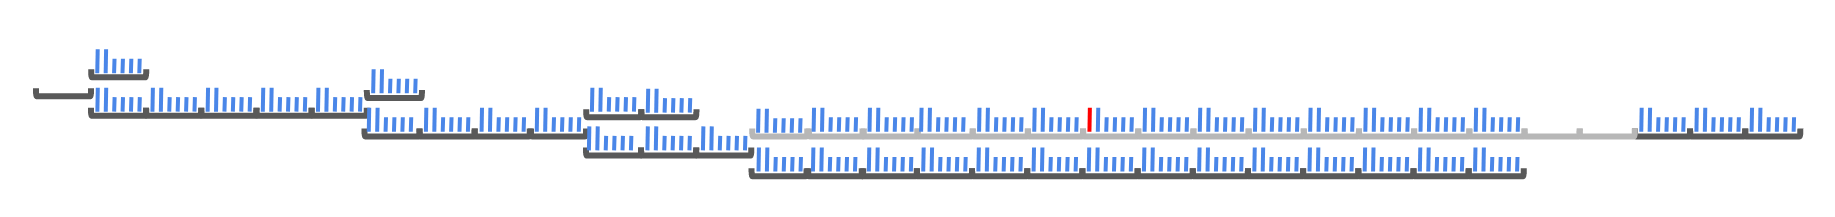
\includegraphics[width=1.0\textwidth]{vis_blocksegment_forking_reorg_txs.png}
\caption{Block composition of a large reorg (eg. finality attack) including
transactions.
  The `fraudulent` modified or omitted (censored) transaction is red.
  %should we identify the transaction on the fork that empties the address from 
which the double-spend was made?
}
\label{fig:blocksegment_forks_reorg_txs}
\end{figure}

\begin{figure}[tph]
\centering
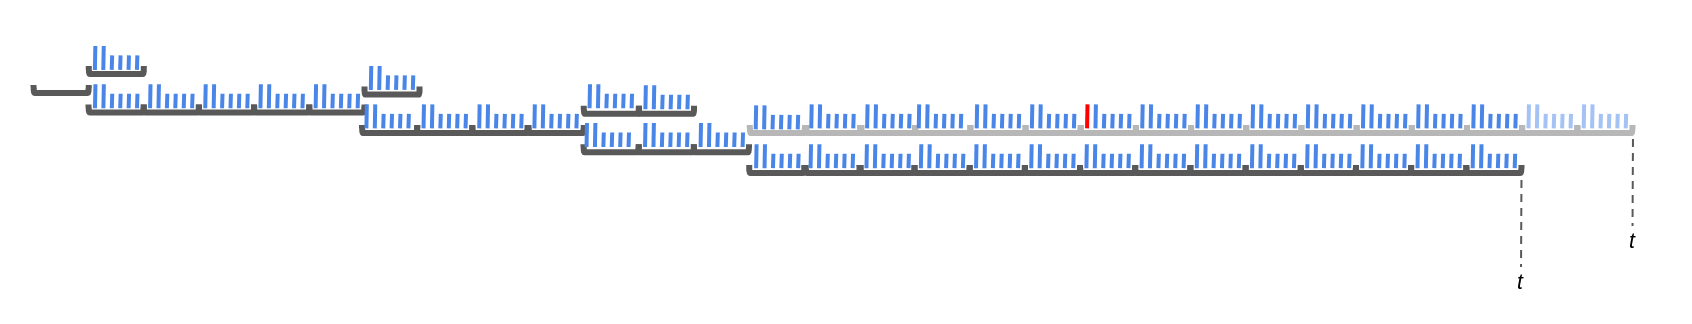
\includegraphics[width=1.0\textwidth]{vis_blocksegment_forking_reorg_t.png}
\caption{Block composition of a large reorg (eg. finality attack), noting a
value $t$ representing some point in time.
Since the domain of this visualization is (implicity) block number, we deduce
that the gray (top) chain has built more blocks per unit of time than its
counterpart.
The value of time $t$ in this case can be understood as an arbitrary instant
where the segments (via their head blocks) are evaluated for canonical status.
}
\label{fig:blocksegment_forks_reorg__t}
\end{figure}

\begin{figure}[tph]
\centering
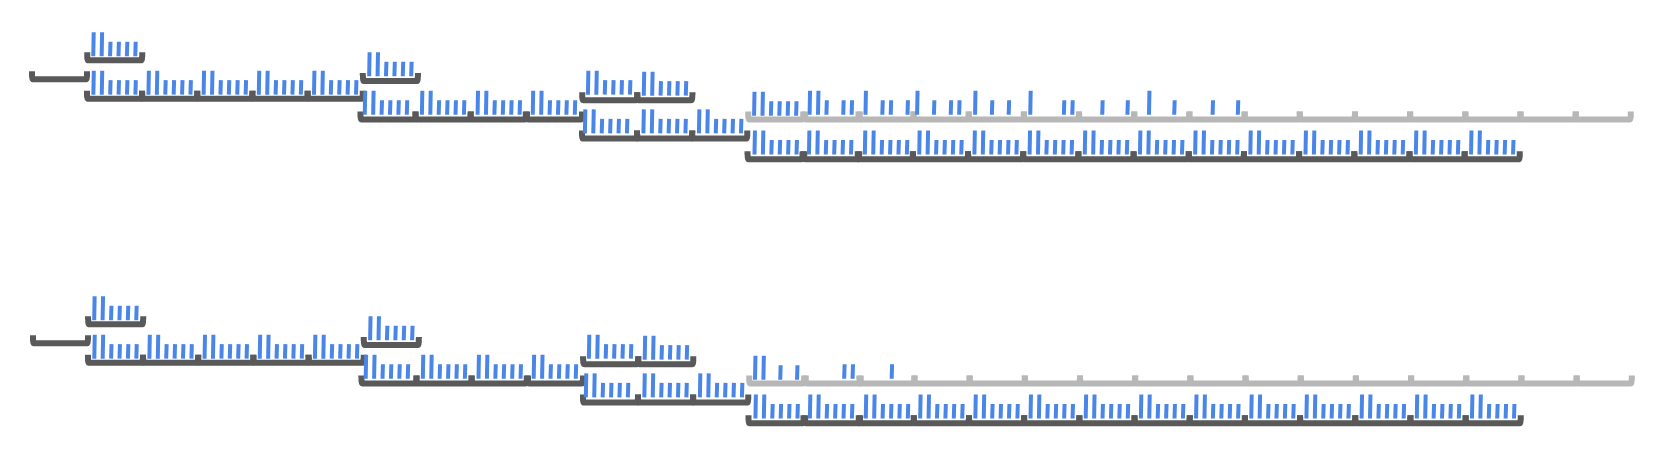
\includegraphics[width=1.0\textwidth]{vis_blocksegment_forking_reorg_anchash.png
}
\caption{Two illustrations of transaction inclusion under the large reorg
scenario and assuming successively aggressive $\tau$ rates (composite frequency
and value of the proposed Transaction Ancestor Hash field and validation).
}
\label{fig:blocksegment_forks_reorg_anchash}
\end{figure}

\begin{figure}[tph]
\centering
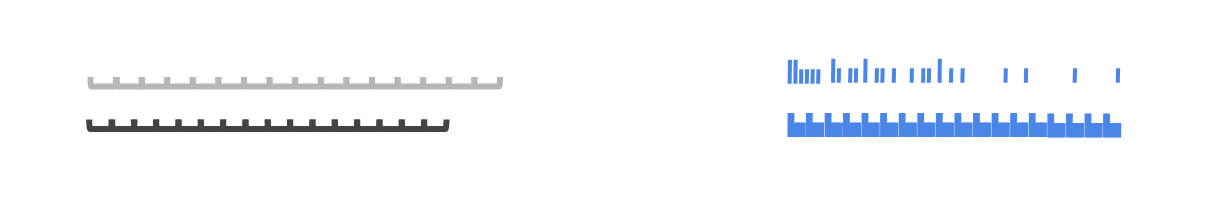
\includegraphics[width=1.0\textwidth]{vis_blocksegment_canonpref_abstract.png}
\caption{
  A component diagram of block and transaction occurrences under the assumed
reorg scenario with transactional Ancestor Hash use.
}
\label{fig:blocksegment_forks_canonpref_incumbent_ex}
\end{figure}

\begin{figure}[tph]
\centering
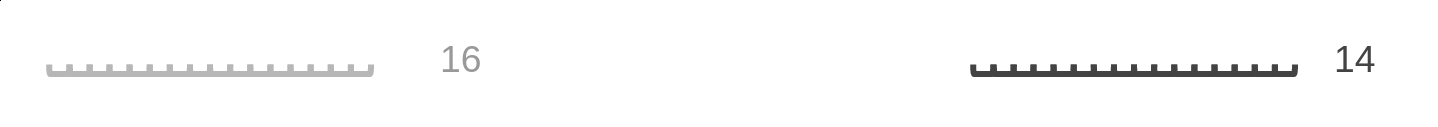
\includegraphics[width=1.0\textwidth]{vis_blocksegment_canonpref_incumbent_ex.png}
\caption{Visual conceptualization of the incumbent canonical-arbitration
initial condition using Total Difficulty values.
}
\label{fig:blocksegment_forks_canonpref_incumbent_ex}
\end{figure}


\begin{figure}[tph]
\centering
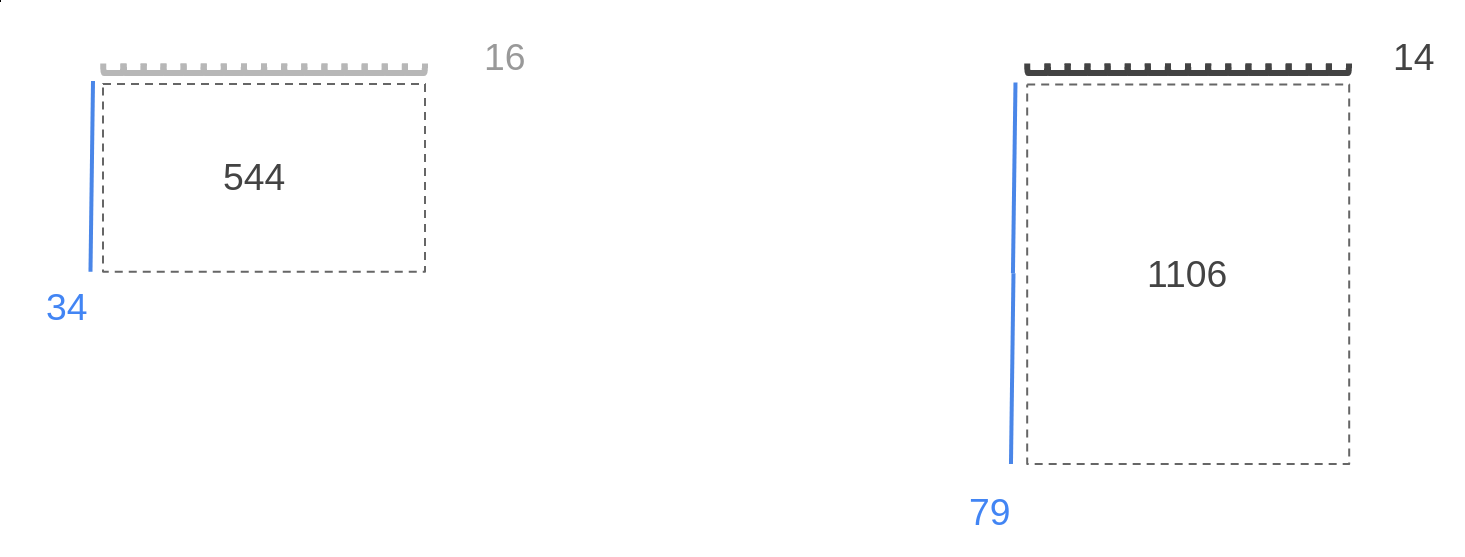
\includegraphics[width=1.0\textwidth]{vis_blocksegment_canonpref_proposed_ex.png}
\caption{Visual conceptualization of the proposed canonical-arbitration initial
condition using Difficulty and TABS values.
}
\label{fig:blocksegment_forks_canonpref_proposed_ex}
\end{figure}

\begin{figure}[tph]
    \label{go-block-step-cdf-interval}
    \centering
    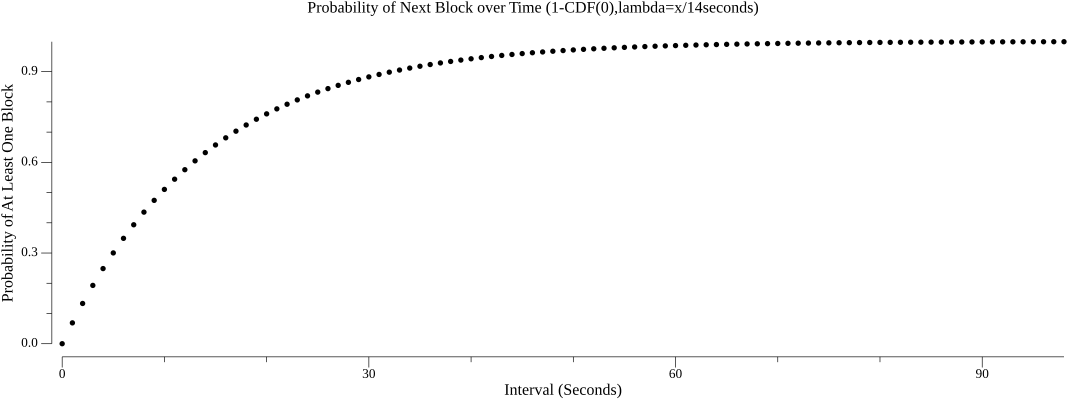
\includegraphics[width=1.0\textwidth]{go-block-step/out/vis_poisson_cdf_next_in_interval.png}
    \caption{
      A Poisson CDF function is used to model the probability of a block
ocurrence (Y) in some interval (X).
      This plot is produced by the included Go test
\texttt{TestPoissonCDFNextBlock}.
    }
\end{figure}


\pagebreak
\section{\normalsize{Theoretical Models}}

%% What is finality?
%% The chance that the blocks you see are permanent.

%% Miner logic.
%% Consensus algorithm block (state) arbitration.
%% Selfish deviance.

\subsection{\normalsize{Miner Expected Revenue}}

We naively define miner expected revenue over time $t$ (in seconds) as:

\newcommand{\minerHashrate}{Miner_{h/s}}
\newcommand{\networkHashrate}{Network_{h/s}}
\newcommand{\blockReward}{Block_\mathrm{reward}}
\newcommand{\blockTransactionFees}{Block_\mathrm{tx_fees}}

\begin{equation}
\frac{\minerHashrate}{\networkHashrate}
\times
P(E,t)
\times
P(C)
\times
(\blockReward + \blockTransactionFees)
\end{equation}

(Note that the ratio $\frac{\minerHashrate}{\networkHashrate}$ is intuitive but
naive, and can be further developed.)

\subsection{\normalsize{Probability of block production}}

We assume that the distribution of block intervals at the network level can be
modeled as a Poisson Distribution.\nolinebreak
\footnote{
One must note that while it may be granted that the model fits \emph{recorded}
network block interval data, it may not necessarily represent the \emph{actual}
production intervals. Neither must it represent accurately the production
interval of blocks by any subset of miners.
}
From this, we can define the probability of any block being discovered in an
interval of $t$ seconds as a derivation of the Poisson CDF.

\begin{equation}
P(E,t) \equiv 1 - e^{-\lambda} \times \sum_{i=0}^{|k|}{\frac{\lambda^{i}}{i!}} 
\end{equation}

In this model, $k$ is held constant at $0$ signifying the occurence of 0
blocks, and $\lambda$ can be defined as the product of an average event rate
$r$ and some time interval $t$.\nolinebreak
\footnote{
For example, given an average network block intervals of $14$ seconds, the
expectation that a next block occurs within $3$ seconds becomes $\lambda =
(1/14) * 3$, yielding $19.2\%$.
The plot in Figure 17 shows this probability for intervals of 0 through 99
seconds assuming an average block interval rate of 14 seconds.
}

\subsection{\normalsize{Probability of a block's canonical state}}

The probability (at the network level) of a block being ultimately accepted as
canonical by the network:

\begin{equation}
P(C) \equiv 1 - \epsilon
\end{equation}

In this simple definition, $\epsilon$ represents the frequency in which a miner
authors a valid (eligible,candidate,potentially-canonical) block which is not
ultimately accepted into the public canonical chain.\footnote{The solutions
these blocks represent in a PoW chain have material cost; ie. wasted
electricity and wasted money.}

We claim and show that $\epsilon > 0$. We take $\epsilon < 1$ for granted as
common sense; canonical blocks exist.

A practical value of $\epsilon$ can be approximated by an empirical measurement
of a network's Uncle rate.\nolinebreak
\footnote{
  There is a lot to say about this, and the nuances of this idea are important
for understanding what kind of approximation this is, and what its limits are.
  A few brief statements are provided for context below, but should not be
considered comprehensive or definitive:

  The Uncle rate represents a record of the existence of blocks which are not
canonical.
  Iff the revenue for those non-canonical blocks is less than their cost of
production, the existence of any non-canonical blocks implies waste, which
suggests a production inefficiency and an economically undesirable
characteristic.
  From this, understanding that the uncle records provided on chain are
potentially incomplete records of the existence of non-canonical blocks.

  %% TODO
  We might explore this further by look at the rewards more closely.

  Is it actually reasonable for a miner to record an uncle, getting the
  other miner paid? Or are uncles only recorded when the author of the
  canonical block is also the author of the uncle?
}
Alternatively, we can derive a reasonable definition of $\epsilon$ using purely
theoretical models, as follows.

Given our assumption of the Poisson Distribution fit for network block
intervals, we can set Poisson's $k$ to 2, representing the occurence of 2
blocks.
Using the Poisson Probability Mass Function, we see that given an average block
interval of $1/14$ seconds, the probability of seeing $k=2$ blocks in some
interval $t=1$ seconds
($\lambda=\mathrm{rate}*\mathrm{interval}=1*\frac{1}{14}$) is:

\begin{equation}
  \frac{\frac{1}{14}^{2}e^{-\frac{1}{14}}}{2!} = 0.00237516...
\end{equation}

But we must extend this to represent the probability of seeing $2$ \emph{or
more} blocks.
We approximate a generalization, using $99$ as an arbitrary upper limit for the
considered number of potential blocks\footnote{The number of potential blocks
is the number of miners on the network.} occurring in the interval:

\begin{equation}
  \sum_{k=2}^{99}\frac{\frac{1}{14}^{k}e^{-\frac{1}{14}}}{k!} = 0.002432736...
\end{equation}

Since by definition the canonical state is applied exclusively to 1 of
$\geq 2$ block occurrences, we have shown that even under an idealized game,
the theoretical $\epsilon$ value is probably a positive, small, number.

While this model could be taken further, for the sake of argument it is not
necessary and will not be pursued.

%% %%%%%%%%%%%%%%%%%%%%%%%%%%%%%%%%%%%%%%%%%%%%%%%%%%%%%%%%%%%%%%%%%%%%%%%%%%%%%%%%%%%%%%%%%%%%%%%%%%%%%%%%%%

\section{\normalsize{Models and Data}}

\subsection{\normalsize{Comparison of a Naive Model and Derived Data}}

If we assume that the characteristics of a Poisson Distribution model represent
accurately the characteristics of the PoW block emission model,
we are lead by reason to compare a theoretical model with empirical data.

We assume that the empirical block interval data is accurately represented in
Figure 18,
and we assume the Ethereum network's mean block interval is reasonably
considered as 14 seconds for the sake of the argument.

\begin{figure}[tph]
    \centering

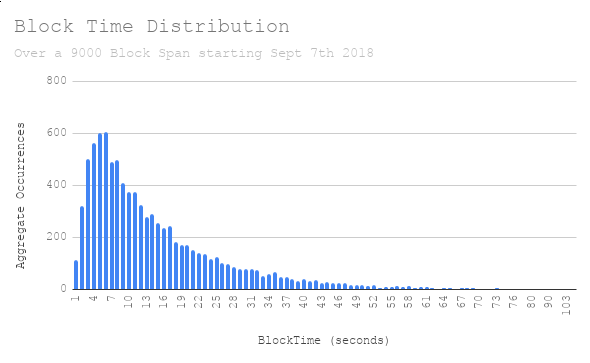
\includegraphics[width=1.0\textwidth]{vis_data_blockinterval_distribution.png}
    \caption{
      Exemplary block interval data for
Ethereum.\footnote{https://ethresear.ch/t/deep-dive-into-current-pow-difficulty-
adjustment-algorithm-and-a-possible-alternative/5267}
    }
\end{figure}

Next, we use a computer program to simulate block intervals under the Poisson
model:\footnote{\texttt{TestPoissonIntervals}}

\begin{figure}[tph]
    \label{vis_poisson_samples_events_86400}
    \centering
    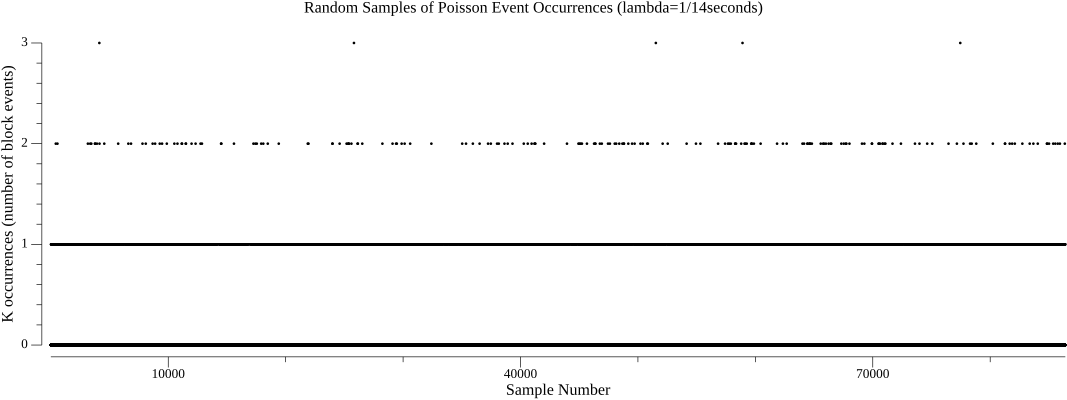
\includegraphics[width=1.0\textwidth]{go-block-step/out/vis_poisson_samples_events_86400.png}
    \caption{
        Procedurally generated event occurrence samples from a Poisson distribution
        with $\lambda = \frac{1}{14}$, sample size of 86400.
        We can interpret the data points at $y=2$ in Figure 20 and Figure 21 as
        representative of occurrences of forks having 2 candidate blocks.
        For $y=3$, the sample has 3 candidate blocks, etc.
    }
\end{figure}

\begin{figure}[tph]
    \label{vis_poisson_samples_eventintervals_hist}
    \centering
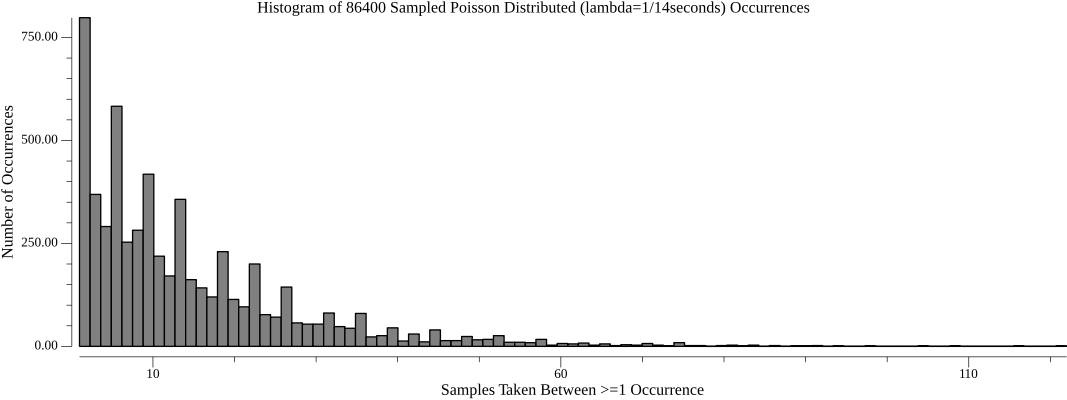
\includegraphics[width=1.0\textwidth]{go-block-step/out/vis_poisson_samples_eventintervals_hist.png}
    \caption{
      Procedurally generated intervals of samples where events $\geq 1$ from
        a Poisson distribution with $\lambda = \frac{1}{14}$.
    }
\end{figure}

%The  represents derivative data from original sample values presented in
%the following plot, Figure 20.

%The same program is reused with a smaller sample size to produce a data set
%(shown in Figure 21) making the intervals between $r >= 1$ occurrences (for
%time interval 1 second) more observable:
%
%\begin{figure}[tph]
%    \centering
%    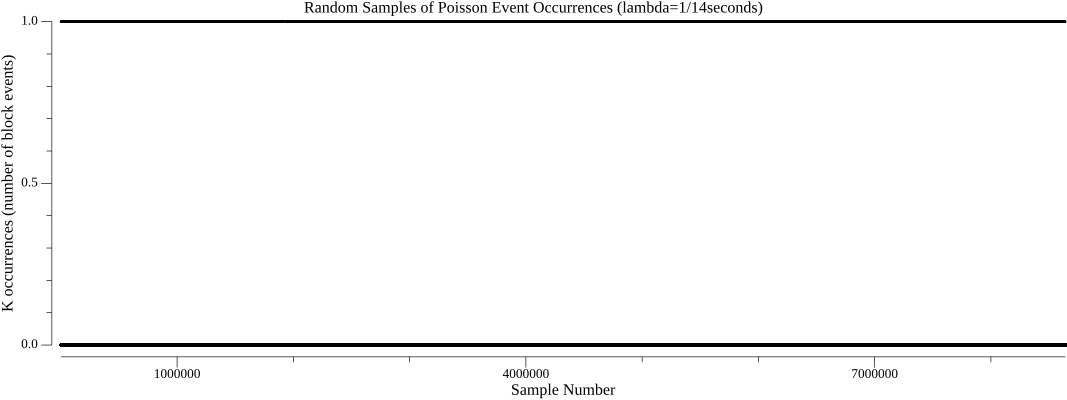
\includegraphics[width=1.0\textwidth]{go-block-step/out/vis_poisson_samples_events_8640000.png}
%    \caption{
%      Procedurally generated event interval samples from a Poisson distribution
%with $\lambda = \frac{1}{14}$, with a sample size of 8640000.
%    }
%\end{figure}

\pagebreak

\textbf{Where is the hump?}

The empirical data clearly shows a `hump` which is not visible in the
procedurally sampled Poisson distribution values,
which instead consistently slope downwards from lesser intervals to greater.
From this simple napkin comparison, we must conclude that our model is as yet
incomplete (or wrong!).

\subsection{\normalsize{Network latency ($\eta$)}}

We propose that an explanation can be made for this mismatch presented in the
previous section between map and territory by a consideration of network
latency.

\vspace{5mm}
\begin{proposition}
  Latency exists.
\end{proposition}

The material existence of network latency is irrefutable under
current physical models of the world.
Information cannot travel faster than the speed of light, which is finite.
The networks in question assume the transmission of messages (information), and
thus, this takes time.
This is latency; the time required for message transmission.

The production of any block depends on the block it will be appended to; its
Parent.
A miner can only begin mining block $B_{i=n}$ after observing block $B_{i=n-1}$.
The existence of network latency as a positive value has already been asserted.

Arbitrarily defining network latency as a constant $\eta=3$ seconds allows us
to produce a revised histogram of expected Poisson event intervals.

\begin{figure}[tph]
    \centering
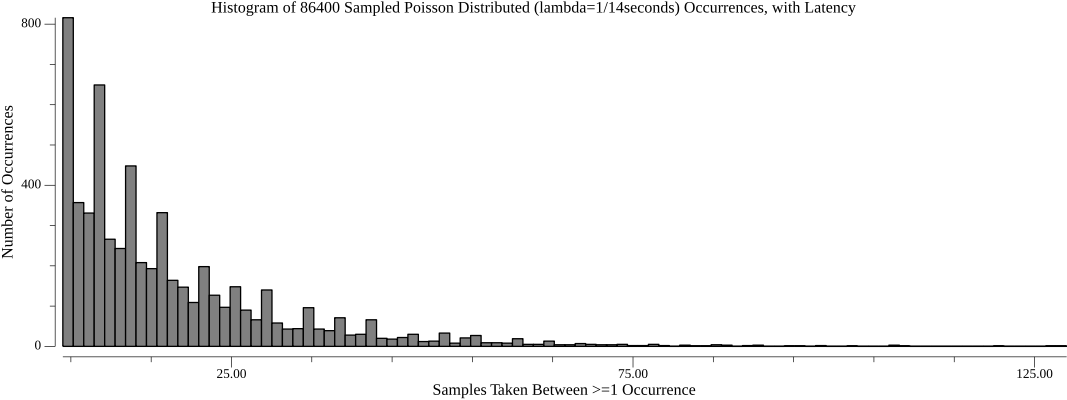
\includegraphics[width=1.0\textwidth]{go-block-step/out/vis_poisson_samples_eventintervals_latencynaive_hist.png}
    \caption{
      Procedurally generated events $k \geq 1$ interval samples from a Poisson distribution
with $\lambda = \frac{1}{14}$, with a sample size of 86400.
      Every interval is increased by $\eta=3$ seconds.
    Clearly, this general application of latency is insufficient.
    The shape is unchanged; only the domain is shifted by $3$.
    }
\end{figure}

\vspace{5mm}
\begin{proposition}
  Latency is heterogenous.
\end{proposition}

If we assume there exist $m$ miners on the network, and that each miner 
controls $\frac{1}{m} \times \networkHashrate$, we can estimate the rate of the 
same miner producing blocks $B_{i=n}$ and its child $B_{i=n+1}$ as 
$\frac{1}{m}$.
When a miner produces both the Parent and Child blocks, the $\eta$ value for
that interval should approach $0$; where time of program execution alone is 
considered relative to the aggregate time of program execution plus network 
transmission duration.
We arbitrarily define $m=8$, and, accounting for this probability, produce 
Figure 23.

\begin{figure}[tph]
    \centering

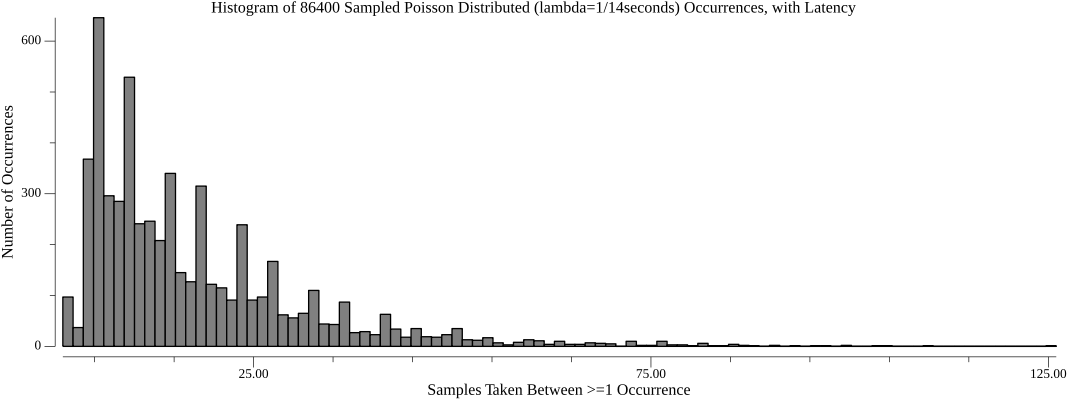
\includegraphics[width=1.0\textwidth]{go-block-step/out/vis_poisson_samples_eventintervals_latencysamesame_hist.png}
    \caption{
      Procedurally generated events $k \geq 1$ interval samples from a Poisson distribution
with $\lambda = \frac{1}{14}$, with a sample size of 86400.
      Every interval is increased by $\eta=3$ for approximately
$1-\frac{1}{8}$ of the intervals.
    }
\end{figure}

Though still naive, we have found a hump.

\vspace{5mm}
\begin{proposition}
  Latency's heterogeneity depends on miner hashrate. %% , and thus, the $\frac{1}{m}$ model is inaccurately simplistic.
\end{proposition}

We assume that miner hashrate for the Ethereum network is unevenly distributed.
This assumption causes our estimation above of Parent/Child same-miner events
as $\frac{1}{m}$ to be inaccurate.
Under this theoretical model, we do not pursue further revisions for this
approximation.

\vspace{5mm}
\begin{proposition}
  Latency may be optional.
\end{proposition}

If latency is defined as the time between transmission and reception of a
message, it attributes should be mostly attributable to physical or
otherwise 'external' limitations.\nolinebreak\footnote{
e.g Cable size, net neutrality (or lack thereof).
}

However, if we were instead to define latency as the time between the availability
of the message (to the transmitor) and the time of message reception,
a new variable arises: delay.

By creating a delay on purpose, a miner gives themselves a head-start
on the mining of a next block. They postpone the transmission of their message,
stalling the game for the rest of the network. While this strategy can benefit
the miner, it comes with the risk that another miner may produce (or have
produced) a competitor block in this interval reducing their chances of success.

On this topic, the reader should reference Eyal and Sirer\footnote{TODO}, who
show that large-hashrate miners (ie. 25\%, 33\%, etc.) can be reasonably
expected to demonstrate this behavior, and with it, a block emission
rate superlinear to their hashrate ratio. They propose network bifurcation
(via a simulated coin-toss) as a network protocol strategy for mitigating
this incentive.

\begin{figure}[tph]
    \centering

    \includegraphics[width=1.0\textwidth]{go-block-step/out/vis_poisson_samples_eventintervals_latencysamesamestrat_hist
    .png}
    \caption{
        Procedurally generated events $k \geq 1$ interval samples from a Poisson distribution
        with $\lambda = \frac{1}{14}$, with a sample size of 86400.
        Every interval is increased by $\eta=3 + \frac{1}{8} \times \mathrm{interval_{\Delta}}$ seconds for approximately
        $1-\frac{1}{8}$ of the intervals.
        This represents a loose event interval model including selfish miner delays.
    }
\end{figure}

%% Let's compare them!

%begin{figure}[tph]
%\centering
%
%
%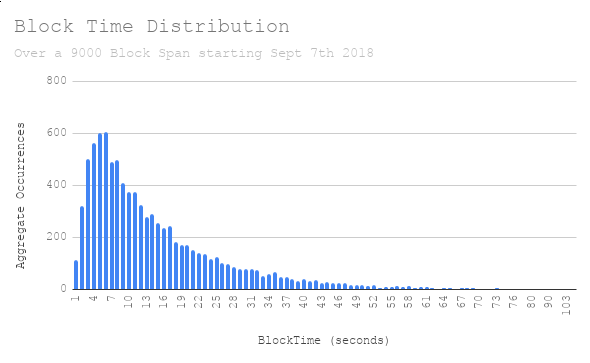
\includegraphics[width=1.0\textwidth]{vis_data_blockinterval_distribution.png}
%\caption{
%    Exemplary block interval data for
%    Ethereum.\footnote{https://ethresear.ch/t/deep-dive-into-current-pow-difficulty-
%    adjustment-algorithm-and-a-possible-alternative/5267}
%}
%\end{figure}

%% %%%%%%%%%%%%%%%%%%%%%%%%%%%%%%%%%%%%%%%%%%%%%%%%%%%%%%%%%%%%%%%%%%%%%%%%%%%%%%%%%%%%%%%%%%%%%%%%%%%%%%%%%%

\section{\normalsize{A Different Model}}

The program \texttt{main} in \textit{go-block-step/main.go} does not use
a Poisson library or algorithm.
Instead, mining is simulated.
Search efficacy per miner is parameterized by network relative hashrate.
The code relies on an arbitrary interval as the space from which a random needle
is drawn. See code comments for more information.

This coded model can be used to simulate network block emission, constant latency\nolinebreak
\footnote{This is less of a concern than it may seem at first glance.}, and
block authorship data.

The model coded does not generate a blockchain. The model, instead,
generates sample information for a single step (block increment)
in the subtree, where the (assumed) parent block is held constant.
Each sample is called a \texttt{round}.

%\begin{wrapfigure}{r}{0.3\textwidth}
\begin{figure}[tph]
    \centering
    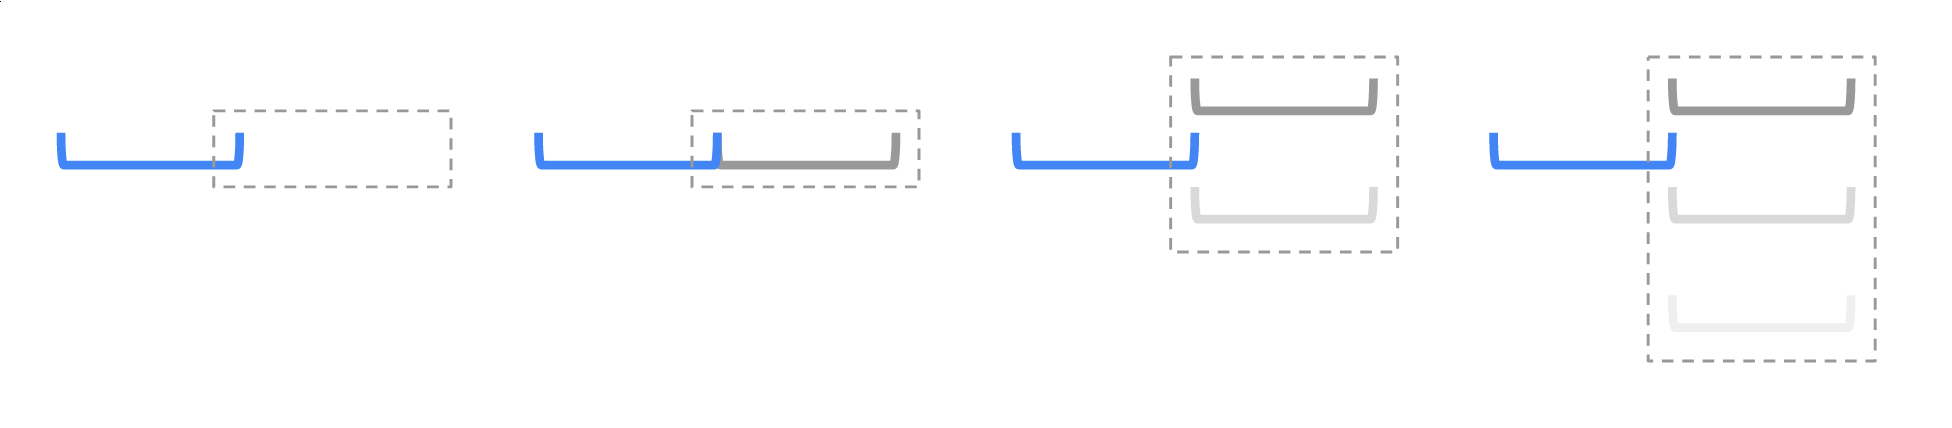
\includegraphics[height=3cm]{vis_theoretical_block-space.png}
    \caption{
        Visualizing theoretical outcomes for a block-space for some time interval
        $t$. The assumed existing parent block is blue.
    }
\end{figure}

For each round, the program is structured to assume a (any) sufficient $t$ such
that at least one child block is produced. This $t$ value is pseudo-random, and
is driven by the pseudo-randomness of the competing simulated miners.
This $t$ value is recorded as, and here referred to, as the resulting
\textit{interval} value.

Notably, the model does not use $H_d$ (header difficulty) values.
So long as we understand that the samples generated do not represent a continuous
chain, we find that assuming a constant arbitrary $1$ value for the
parent $TD$ value is reasonable.

Our aim is to model block emissions in a pseudo-statistical way,
focusing on game theoretical decisions for miners rather than
block-network propagation or network shape.

Latency is modeled only to the extent that it impacts block production
intervals. A constant value is used; added to the recorded block interval
for any miners who (probabilistically assigned) did not mine the
parent block.

%This is, for example:
%
%  - Parent/Nothing \\ %% Blockchain turns off. Probably happens often.
%Unmeasured.
%  - Parent/Child \\
%  - Parent/Child,Child (twins/pending ommers|potential uncles,a fork,a
%bifurcation
%(of network consensus)) \\
%  - Parent/Child,Child,Child (triplets...a trifurcation (right!?))
%

%Another way to think of this is that the model replays the occurrence of the
%production of a single 'block-space' on the network (again, where the term
%block-space signals that zero \emph{or more} blocks could occupy the space (for some
%arbitrary interval unit, eg. $1$ second or $1$ milliscond, etc.). Necessary
%block values are held constant for an otherwise imaginary parent block.
%
%The aim of this paper intends specifically to deflect itself such as to entirely
%miss the mathematical aspects of graph theory or network algorithms, of which
%the author of this paragraph happens to have nearly exactly zero knowledge.

We could introduce a small bit of randomness to the latency value, but that
would only produce noise.

We can play with latency. The program wants it to be understood as a tuneable
parameter. For now, the program knows that same-author rounds add a latency of
zero, while everyone else adds a constant legacy value
\texttt{RoundConfiguration.Latency}, which is, as you guessed, configurable per 
round.

We know that latency is an important thing.
We assume, however, that the latency economy is efficient and nearly usally 
optimized,
and that non-negligible-hashpower-share miners will be able to cost-effectively
purchase sufficiently competitive latency values. With this, we assume that
these same miners have approximately probably pretty much the same latencies.

The model could be extended or modified to do latency differently.

The model could also be changed to do hashrates and puzzle interval
approximation differently.

Implementation of a stateful block difficulty characteristics would enable
representation of random walk information concerning network relative hashrates
for miners. This would be more realistic, but would also be more noisy.



The information generated is not deterministic.

\textbf{Data}


\begin{figure}[tph]
    \centering
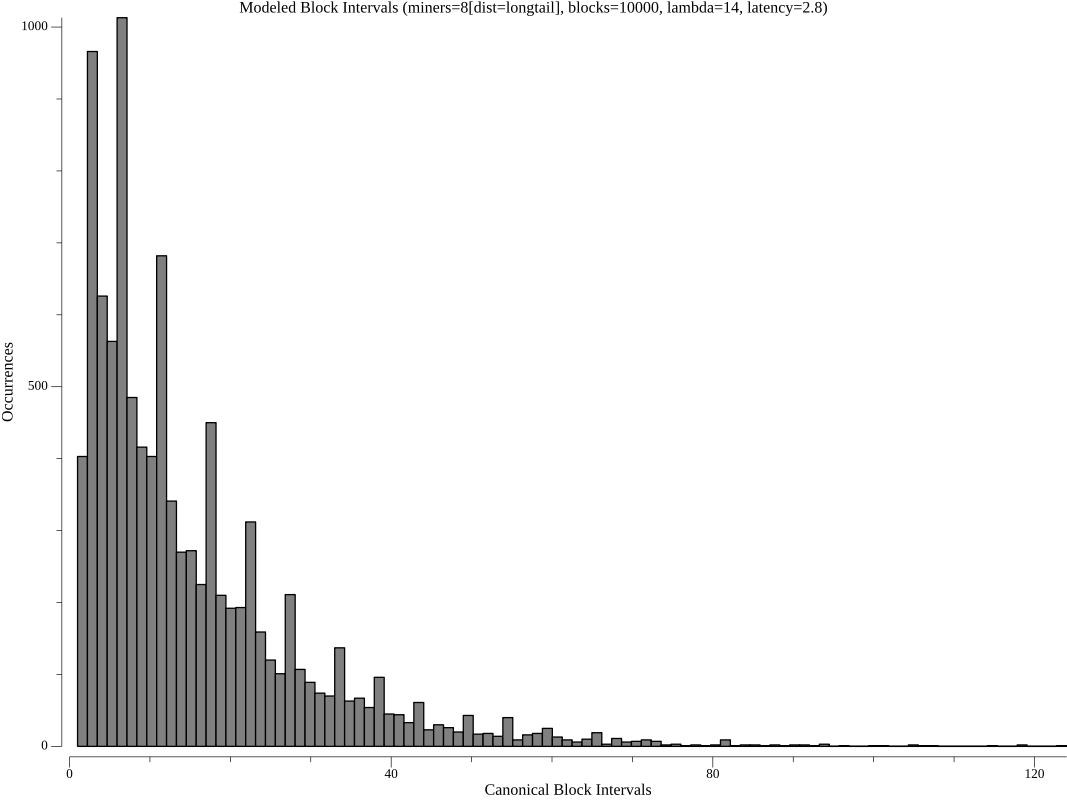
\includegraphics[width=1.0\textwidth]{go-poisson_A0_blockIntervals.png}
    \caption{
      Simulated block intervals for $\lambda=\frac{1}{14}$, $\eta=2.8$, with
      $8$ miners, each with procedurally generated long-tail-ish shaping
      relative hashrate shares.
    }
\end{figure}

\pagebreak

The first \texttt{Round} generates a print out:

\begin{verbatim}
CONFIG

Name:             A, ConsensusAlgorithm: TD,
NetworkLambda:    14, Latency:          2.80,
TickMultiple:     1, Rounds:           10000,
NumberOfMiners:   8, HashrateDistType: longtail,

GENERATED MINERS

Number: 8, Distribution: longtail, Hashrate Checksum OK:    true,
Hashrates: [0.333 0.222 0.148 0.099 0.066 0.059 0.044 0.02]

INTERVALS

Mean: 15.8650,
Med: 11.8000, Mode: [3.8000],
Min: 1.0000, Max: 139.8000,

ELIGIBLE AUTHORS PER BLOCK

Mean: 1.0819,
Med: 1.0000, Mode: [1.0000],
Min: 1.0000, Max: 3.0000,

MINER CANONICAL WINS

miner=0 hashrate=0.333 winrate=0.338 winrate/hashrate=1.013 (3375)
miner=1 hashrate=0.222 winrate=0.227 winrate/hashrate=1.020 (2266)
miner=2 hashrate=0.148 winrate=0.143 winrate/hashrate=0.963 (1427)
miner=3 hashrate=0.099 winrate=0.097 winrate/hashrate=0.979 (967)
miner=4 hashrate=0.066 winrate=0.066 winrate/hashrate=0.998 (657)
miner=5 hashrate=0.059 winrate=0.060 winrate/hashrate=1.022 (598)
miner=6 hashrate=0.044 winrate=0.043 winrate/hashrate=0.982 (431)
miner=7 hashrate=0.029 winrate=0.028 winrate/hashrate=0.953 (279)

\end{verbatim}
\pagebreak
\begin{verbatim}

ANALYSIS

Ticks: 136550, Rounds (Blocks): 10000, Ticks/Block: 13.655
AuthorSameParentChildTally/Block: 0.211
ArbitrationDecisiveRate: 0.028, ArbitrationDecisiveTally: 277
ArbitrationIndecisiveRate: 0.052, ArbitrationIndecisiveTally: 522

\end{verbatim}


\section{\normalsize{Interlude: In Consideration of the Tick}}

We have, until now, taken arbitrary rates, specifically \emph{rate units} for 
granted.

Ethereum formally defines\footnote{Ethereum Yellow Paper} block timestamps as:

\hypertarget{block_timestamp_H__s}{}$H_{\mathrm{s}}$ is the timestamp (in 
Unix's time()) of block $H$ and must fulfil the relation:
\marginpar{Ethereum Yellow Paper}
\begin{equation}
H_{\mathrm{s}} > {P(H)_{\mathrm{H}}}_{\mathrm{s}}
\end{equation}

This mechanism enforces a homeostasis in terms of the time between blocks; a 
smaller period between the last two blocks results in an increase in the 
difficulty level and thus additional computation required, lengthening the 
likely next period. Conversely, if the period is too large, the difficulty, and 
expected time to the next block, is reduced.

Timestamps are otherwise arbitrary.

Time in the real world moves with apparently infinite fluidity. An instant of
time is as small as the instance of a Cartesian point.

Time in computers is as small as the time it takes for information to move.
This is a bigger number than the theoretical instant.

Time in Ethereum gets as small as $1$ second.
The \texttt{go-ethereum} network client program \texttt{geth}\footnote{The 
majority share client on the Ethereum network}, ignores (does not process) 
blocks having a timestamp $B_s > now() + 15$. This is a normally undocumented 
subjective behavior, parameterized by some computer's clock. Running
\texttt{geth} on a computer with a clock set 'late' (reading actually past 
values) will fail to maintain synchronisation (consensus) with the network.

In coding a simulation, we can arbitrarily scale a \textit{tick} interval,
representing some arbitrary atomic unit of time corresponding to a program step 
or loop. The tick parameterizes the time domain of the simulation.

Since much of our work here assumes the job of fitting a model to the empirical
information available, we need to acknowledge the limits of this approach.

Our empirical knowledge is constrained (at this point in the research\footnote{
For both practical and theoretical reasons.}) by using exlusively \emph{
objective} measurements. Block timestamps are objective measurements.
If we were to take our own readings of network latency, or of block production
intervals (for example, by actually mining and recording measurements), these
would be what this paper considers \emph{subjective} data.

We do not consider any empirical information with time units less than $1$
second. Our programming can be configured to represent a simulation of
arbitrary time units. Evaluation of the degree of fit between model and
data should take this into consideration.

%% %%%%%%%%%%%%%%%%%%%%%%%%%%%%%%%%%%%%%%%%%%%%%%%%%%%%%%%%%%%%%%%%%%%%%%%%%%%%%%%%%%%%%%%%%%%%%%%%%%%%%%%%%%

\section{\normalsize{Model Comparison: Fork Rates}}

We have now two models which can be used to estimate fork rates during
simulated chain growth. We compare the information provided by these models with
empirical data.

We are concerned with fork rates because a fork represents, by definition, an
instance of reduced finality. Only one block per block number can be ultimately
considered canonical; the others will become obsolete (impermanent).

The ambiguity of \emph{which} block shall become canonical is a matter of
network, and miner, efficiency. Time and energy spent on impermanent blocks is 
wasted.

We note further, that the cost of forks are not limited to the two (or miner)
beneficiary authors of those blocks. We can consider, as an example, that each
of two miners broadcasts their candidates to the network nearly simultaneously.
Attributed to network latencies and graph shapes, the network consensus bifurcates
and global hashrate is halved (each miner having won-over half of the network).
At this point 50\% of network hashpower will be ultimately wasted; only one
side of the fork will ultimately become canonical. The cost of the ambiguity is
borne by all players (though not necessarily fairly distributed).

This assumed state of ambiguity of the candidate blocks is the result of the
canonical arbitration algorithm. A canonical arbitration algorithm yielding a
lower ambiguity rate will reduce the network's block emission waste and improve
expectations of permanence for the overall chain state.

\subsection{\normalsize{Simulated Fork Rates vs. Empirical Uncle Rates}}

We know that uncle rates represent a theoretical minimum measurement of actual
orphaned block rates; the orphans \emph{may} be recorded but are \emph{not
necessarily}.

Can we use an economic model of the incentives of orphan records to suggest to
what degree empirical uncle block rates suggest a complete record?
If miners are not incentived to record orphans they do not mine themselves,
then the recorded orphans will omit those. On the other hand, if it is
profitable for the miner to record orphans regardless of their author, then we
should expect the record to be more complete.

The revenues from orphan recording are inuitive; they are clearly defined and
scaled to the block reward. They are positive. But what are the costs of
recording an uncle?

Total network Wei supply is assumed to be finite for the sake of
argument.\nolinebreak
\footnote{This is not a guarantee for Ethereum, though it is for Ethereum Classic.}

Since an orphan record benefits the miner of the orphan \emph{more} than it
benefits the recording miner, we are lead to reason that it \emph{may} be that the
cost of distributing \emph{any} capital to competitors dilutes the value of a
miner's own capital.

We leave this line of reasoning open-ended.

For the sake of our proposed model, it is enough to assume an observable
objective measurement (uncle rate), and to handle it as theoretical minimum
proxy for actual fork rate.

We turn to empirical data.

At the time of writing, Etherscan.io\footnote{https://etherscan.io/uncles}
shows $1,207,850$ recorded uncles and a current canonical height of $13,753,436$. 

\begin{equation}
  1207850 / 13753436 = 0.0878217
\end{equation}

We interpret this as representing an orphan rate of about 8.7\%. 

Comparatively, using the \texttt{main} program we simulate a network with
$\lambda=14$, $\eta=1.5$, $8$ miners with hashrates distributed as an
approximate long-tail, at a tick interval representing $100$ milliseconds, over
$10,000$ samples, and yielding a fork rate of 8.39\%. 

Raising latency to $\eta=2$ can raise the rate to 11.7\%.
Alternatively, raising the number of miners to $16$ seems to raise the rate to
around 8.7\%.

It is tempting to manipulate modeled latency values in order to meet the
shape of empirical block interval data. But we must resist this temptation.

We do not know real network latency values, and have no objective way of
measuring them. Further, we expect that even reliably measured subjective values
would vary and are regularly subject to change. This point is especially
pertinent when latency is considered as both mechanically-derived (tube limits) and
arbitrarily decided values (eg. selfish head-start delays).

\begin{wrapfigure}{r}{0.5\textwidth}
    \centering
    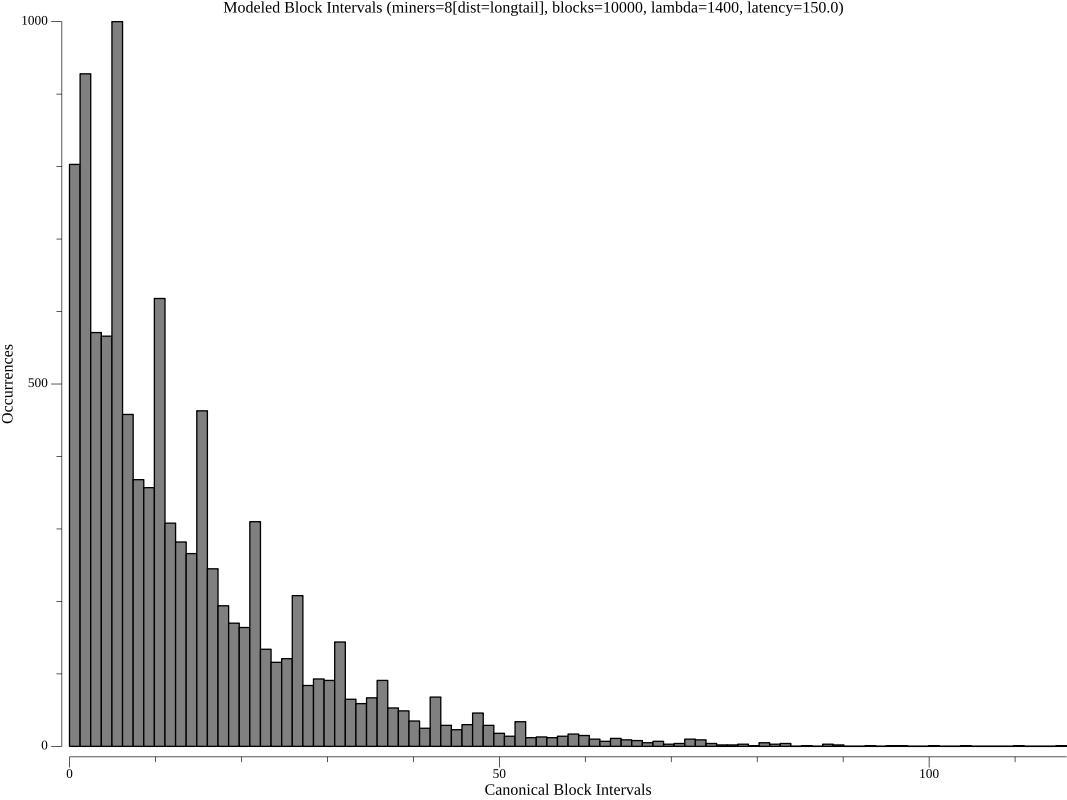
\includegraphics[width=0.5\textwidth]{sim_a_anteater.png}
\end{wrapfigure}

We note, however, that under this simulation, the generated block interval
distribution (Figure right) doesn't seem to match the empirical data.
The intervals are too small.

If we re-prioritize the fit to a back-of-napkin same-shape rubric on block
intervals, a $\eta=4.2$ approximates a better fit (Figure 25, below). At this
latency rate, the model yields a simulated fork rate of approximately 23.5\%.
A Poisson distribution sampling for the same tick duration is overlaid in red.

\begin{figure}[tph]
    \centering
    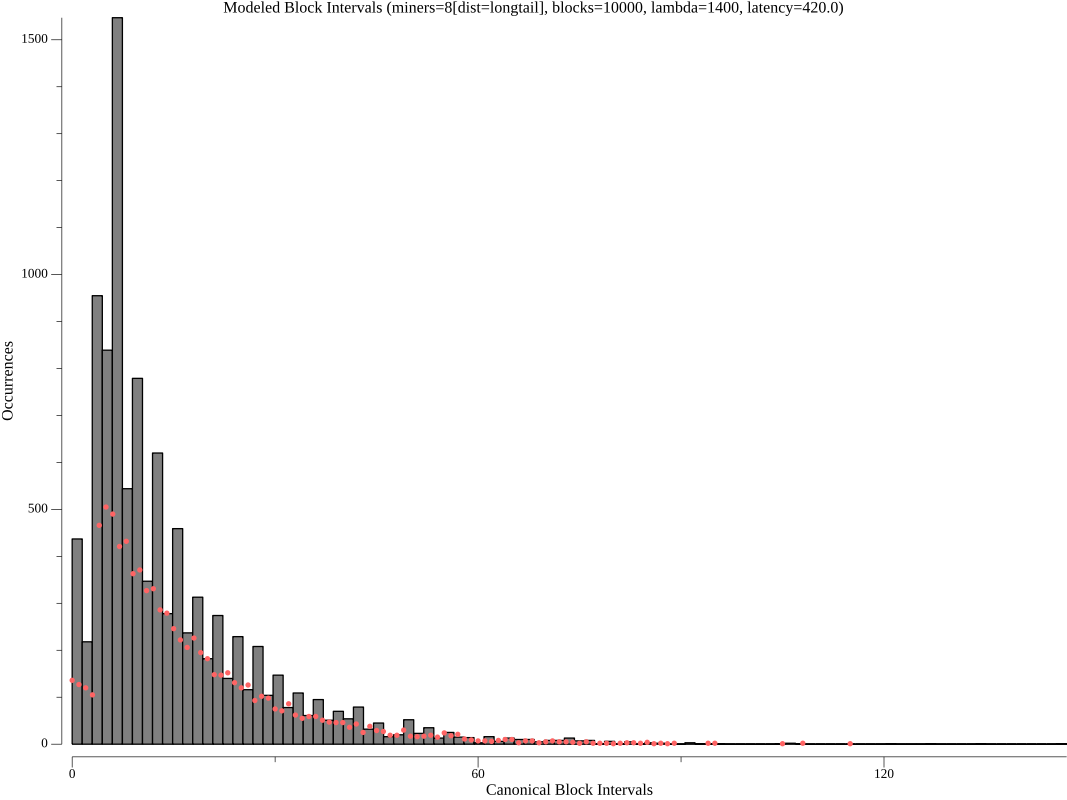
\includegraphics[height=8cm]{sim_a_bravo.png}
    \caption{
      Poisson Distribution interval distribution samples
      overlaid on simulated intervals.
    }
    \label{fig:sim_a_bravo}
\end{figure}

Our intention is not to build a best-fit model for empirical data.

The intention for the model is to adequately theoretically represent the game
which drives the PoW network. With a model that \emph{behaves like} the real
world in its key measurements, we can explore the impact of the proposed
algorithmic modification to the canonical selection logic.

\subsection{\normalsize{
    Comparing Simulated Fork Rates:
    Proposed vs. Incumbent Canonical-Selection Algorithms
}}

When an event $k \geq 2$ occurs, network protocol defines a set of rules for
determining (deciding/arbitrating) canonical status for exclusively one event
(where an 'event' is equivalant to an eligible block).\footnote{
  In fact, the protocol design for canonical-selection is applicable to \emph{all}
  scenarios of canonical-status arbitration between \emph{any} two blocks.
}

We compare the incumbent Total Difficulty (TD) condition with the proposed
Total Difficulty $\times$ TABS (TDTABS) condition by replacing the arbitration
logic used by the model in scenarios (block-space rounds) with $2$ or more
candidate blocks, focusing on the respective rates of 'decidability', where
the condition returns an unambiguous choice for the canonical block.

Under the same conditions of the scenario presented in the previous section,
we find the following exemplary values:

\lstinputlisting[language=]{main_output_charlie.txt}

%Of note here, we find the \textit{ArbitrationDecisionRate} (and
%complementarily, \textit{ArbitrationIndecisionRate}).

The TD model shows a decision rate of 3.9\%, and an ambiguity rate of 3.6\%,
where both rates are measured against total rounds.

The TDTABS model shows a decision rate of 5.1\%, and an ambiguity rate of 2.5\%,
where both rates are measured against total rounds.



%% \comment{
%% In the development and proposition of the canonical-selection algorithm
%% modification, we're interested in a few key features:

%% - Improving finality. \\
%% - Not breaking game theoretical/economic incentives. \\
%% - Not worsening the utility or potential work of the system (ie. same or more
%% possible transaction throughput). \\
%% }


%% \comment{
%% Ethereum rewards the production and recording of uncles.

%% Although the authors are here tempted to dive into the nuances (and history)
%% of uncles, for the sake of the necessary arguments in this paper they will
%% instead assume that
%% While a citation would be nice to suggest that this is common knowledge, we
%% can also use our understanding of Ethereum to derive a rationale of existence
%% of this number, \textit{at least some positive value}, independently.

%% In Ethereum, Uncles is the pet-name/jargon given to forking blocks.
%% Specifically, to the blocks of a fork which do not ultimately wind up being
%% considered canonical.
%% Ethereum rewards the production and recording of uncles. Both the miner of
%% the uncle and of the canonical block (recording it) are rewarded.\nolinebreak
%% %\footnote{
%% Historically, the rewards for uncles and their citations have been changed.
%% In the good old days, Uncles got rewarded a lot more than they are today.
%% Something like $\frac{32-uncleDepth}{32}\mathrm{10^{18} Wei}$ (but don't 
%% quote
%% me on that).
%% Much closer to the reward of the canonical block, and (I believe)
%% benefitting both uncle and canonical miners by equal margin.
%% A lot of uncle blocks got mined.
%% It was kind of a problem. (Or \textit{was it?})
%% Anyways, now, they pay less for orphans.

%% So there are economic incentives to publish, observe, and record uncle block
%% information.

%% And, indeed, uncle block information is published.
%% %% TODO: Cite me.
%% Reliable records of complete uncle block information are, however, imperfect.
%% %% TODO: Say more about why uncle block information is imperfect, and what
%% those shortcomings mean for this analysis.

%% For the sake of argument, we assume from here that Ethereum Uncle rates
%% hover around at least 5\%.
%% }

%% %%%%%%%%%%%%%%%%%%%%%%%%%%%%%%%%%%%%%%%%%%%%%%%%%%%%%%%%%%%%%%%%%%%%%%%%%%%%%%%%%%%%%%%%%%%%%%%%%%%%%%%%%%

\pagebreak
\section{\normalsize{THE REST OF THIS IS UNEDITED CRUFT}}

Here be dragons. Ye be warned.

\subsection{\normalsize{Probability of canonical acceptance of an eligible
block by the network}}

Intuitively (and ideally), this value is 1. 
Empirically, this value is less than 1.

We attribute this to network latencies and network graph shapes.\nolinebreak
\footnote{
Plural forms are used to emphasize that these values are variable.
Both values are difficult to measure objectively with a high degree of
confidence.
}

Scenario:

Blocks are produced independently and simultaneously by at least two miners.
These blocks have equivalent Total Difficulty values and numbers (for the sake
of argument).
We assume that the network is bifurcated (forked). For sake of argument, we
assume 50\% of the network (by hashrate, say) is on one side of the fork, and
50\% on the other.

Assuming `good` data availability is maintained for \textit{the whole network},
we expect that the fork to resolve quickly.
Probably one side of the fork will produce a block quicker than the other,
yielding a subtree with a greater Total Difficulty value than either of the two
forks previously.
This 2-block chain segment is expected to be adopted as canonical as soon as it
is made available to a node.
For 50\% of the network, this will result in a minus-1/plus-2 block reorg. For
the other 50\% who were originally on the eventually-winning segment, no reorg
is required and the next block is appended. Consensus is reached again.

The general case for the expectation of this resolution is the probability of
simultaneous block production in a series of arbitrary length.
If we define the probability of simultaneous block production as $P_s$,
then it follows that the probability of a bifurcation enduring $n$ blocks
(where $n$ must be greater than 0) be $(P_{s})^{n}$.

Next, we must examine more closely the criteria for what has been called
simultaneity.
In fact, we mean `nearly simultaneously`, or `functionally simultaneous`.
We can loosely establish the bounds for this window from assumed (or measured)
network latency values.
Blocks produced independently within some time interval shorter than the
involved network latencies (ie. between the two competing miners)
will cause each miner to deviate from the optimal protocol (mine the best block
available), because while the next best block available will exist at the
network level,
it will not be available to \textit{them} because of the mechanical limitations
of the network.

We have variables defined for this scenario.

$\lambda$ represents network mean block time in seconds.

$\eta$ represents block message latency between two nodes in seconds.

If we assume a Poisson Point Process distribution for the independent miners,
what is the probability expected for 2 independent new-block events to occur
within an interval $\eta$ of each other?


\subsection{\normalsize{Impact of Proposed Algorithmic Condition on Network
Consensus}}

Conceptually, TABS relies on a fundamental assumption: capital is not
distributed evenly.
If we hold transaction availability to miners constant, in order for TABS to be
effective, we must assume that miner balances are not equal.
If all miner balances are equal and transaction/block inclusion is held
constant, TDTABS does not modify the expectations of an incumbent TD-only based
algorithm.

Assume a waste rate for the network of 5\%.
The Ethereum network's current uncle rate is 5\%. We consider this a minimum
value (there could exist unrecorded/unobserved uncles), but all recorded uncles
are observable and valid.
We assume that uncles are economically undesirable (compared to full blocks),
and as such, that their existence is optimized at the lowest level mechanically
possible.
The occurence of an uncle signals an instant of network consensus
undecidability.
An uncle represents a fork.
An indecisive event signals a lower state finality expectation than a decisive
event.
It also signals, for the miners of each twin block, a reduced expected revenue
for that block (since the probability of impermanence is greater than for an
uncontentious block).

We use Digiconomist data from 20211203 claiming 92.42 TWh as Ethereum's
annualized energy
consumption.\footnote{https://digiconomist.net/ethereum-energy-consumption/}

94.42 TWh \rightarrow MWh = 94420000 MWh

We then cite
Wikipedia's\footnote{https://en.wikipedia.org/wiki/Cost_of_electricity_by_source
} data for projected LCOE by 2025 (as of 2020) for US simple average cost for
advanced nuclear energy as \$81.65 / MWh.

94420000 MWh \times \$81.65/MWh \equiv \$7,709,393,000

If TDTABS reduces network block waste from 5\% to 2.5\%, that suggests an
approximate annual global savings of \$192,734,825.




\subsection{\normalsize{When Should Miners Mine on the Next Block?}}

\pagebreak
\section{\normalsize{Rationale}}

\pagebreak
\section{Placeholder}
\subsection{\normalsize{Transaction Ancestor Hash}}

%% %%%%%%%%%%%%%%%%%%%%%%%%%%%%%%%%%%%%%%%
%% %%%%%%%%%%%%%%%%%%%%%%%%%%%%%%%%%%%%%%%
%% %%%%%%%%%%%%%%%%%%%%%%%%%%%%%%%%%%%%%%%
%% \vspace{6cm}
%% %%%%%%%%%%%%%%%%%%%%%%%%%%%%%%%%%%%%%%%
%% %%%%%%%%%%%%%%%%%%%%%%%%%%%%%%%%%%%%%%%
%% %%%%%%%%%%%%%%%%%%%%%%%%%%%%%%%%%%%%%%%

\subsection{\normalsize{Another Thing}}

\pagebreak
\section{\normalsize{Theoretical Analysis}}

This section provides reasoning around the theoretical implications of the
proposed algorithm.




\subsection{\normalsize{Network Behavior Analysis}}

Demonstrate that the `objectivity` characteristic of consensus-facing
information is invariant.
The additional observable data required by the proposed algorithm is chain
data. It is in the same scope (`context`) as data relied on for the existing
canonical-preference scheme.
All nodes can make the same decision given the same information at any point in
time.

Need to show that consensus properties for the network are invariant.

Demonstrate that the incentive to mine the NEXT BEST block (ASAP) is preserved
as an invariant.

Consider also:
- theoretical additional block processing cost (\textit{more} to do)
- necessity of observable chain state (well, only balance) for block
validation. Compare with requirement of Ethash for block validation. Compare
with other validations, eg. Parent Hash, Number.

\section{\normalsize{Game Theoretical Analysis}}

Show the equation of miner predicted (expected) revenue for some (next) block.
Next blocks are uncertain, future events.
We can show the probability of some miner winning the next block as the plot of
the percentage chance of next-block being found over time, divided (scaled) by
their relative hashrate.
We show that for t=0..t=n that the expected revenue of the miner goes up.

We consider this plot for the scenario where a miner observes a next block.

\subsection{\small{Placeholder}}\label{sec: S4.12}

\section{\normalsize{Economic Analysis}}

\section{\normalsize{Practical Analysis}}

This section offers analysis and interpretation of empirical and derived data.

\pagebreak
\section{\normalsize{General Proposition}}

We want to improve chain state finality characteristics without compromising
other security characteristics of PoW network protocol.

We propose the introduction of segment-specific transactions and an accounting
on a representative measure of capital saturation for some segment, yielding a
"hybrid" canonical-score value.

We intend to extend the incumbent PoW canonical-arbitration protocol to include
reasoning about segments' relative "capitalization" rates.
The introduction of such a variable can be shown to raise the expected cost of
an alternative-history-based attack and to have minimal negative side effects.

We get to to keep, and still deeply rely on, an incumbent PoW emission and
consensus pattern.


% Given: \\
% - A non-zero (the more the merrier) rate of transactions on the network. \\
% - A non-zero rate of segment-specific transactions (a "large" $\tau$). \\
% - A 51\%-attack scenario. \\



\section{\normalsize{Open Questions}}

\subsection{\small{What if emissions revenues were separated from tx processing
revenue?}}\label{sec: S4.12}


\subsection{\small{Can we show that 3\%/97\% is a sensible
simultaneous-production rate using just the Poisson emission
model?}}\label{sec: S4.1}

NOTE that we don't assume perfect simultanaeity; the Poisson model forbids this.
We set a window we define as "competitive." We characterise this by a
heterogenous acceptance of blocks at some number at the network-level; blocks
produced near-enough-to-simultaneously to produce a network fork (of some
scale; a point which could be additionally investigated: to what scale? 50\%
partisanship? 0.01\%?), e.g. 300 milliseconds.

\subsection{\small{Can we show formally that it is game-optimized to mine on
the next block immediately (no matter a miner's own anticipated TABS
score)?}}\label{sec: S4.2}

We assume under the standard Pow/Ethash game, that it is optimal to always mine
on the greatest block available.
However, we know that this assumption has limits; "selfish" miners with
sufficient relative hashrate (greater than 25 percent) can/should be expected
to optimize toward their own self interest.

Is the strategy around potential witholding of next-blocks maintained as an
invariant?
Is the strategy around mining the best-available block (vs. continuing work on
a potential own fork) maintained as an invariant?

A miner will be able to calculate their anticipated TABS in advance (before the
finalized production of their next block, depending/awaiting an Ethash
solution).
This leads one to wonder: \\
- If a miner foresees a "+" TABS block of their own (eg. they have receive in
private a large transaction to process, or they are just rich), \\
- after an interval of 3 seconds from its parent, child block from another
miner is broadcast having a "-" TABS value. This creates a block with
CS=(2049*127)/(2048*128). \\
- Is a competitive, "rational" miner incentivized to continue mining for some
period of time in the expectation of discovering a block with a comparatively
greater CS? \\
    - If they discover a block at the 8 second interval (5 seconds later),
their block would have CS=(2049*129)/(2048*128). \\
    - BUT, the competing miners will have had a 5 second "head start" on their
\textit{next} block (n+1).

I think this can be solved by finding the relative area under the PDF curve
(CDF?) of the Poisson distribution for that time interval (the chance of
another block appearing).
This value should then be multiplied with the expected value of that next block
(in CS units).

My intuition is that the CS value of a "whole" block is enough greater than the
marginal differences caused by Difficulty and/or TABS adjustments that time
spent toward that whole cookie is more valuable than chasing crumbs.

To demonstrate this, we can show that the CDF (?) of the Poisson distr. for
lamda=13 gives a 2\% likelihood to a next block at the 1-second interval. This
number is totally made up.
We show that 0.02 * NextBlockCS is greater than the marginal difference
possible with the selfish miners competing block.
So the expected value (after some very small amount of time) is higher for our
potentially-selfish miner to pursue the next block instead of their own.

We could add realistic complexity by noting that our potentially-selfish miner
controls some portion of the network hashrate.
Their decision to pursue a selfish block/fork instead of mining the next-best
block would remove hashrate from that block's potential child, thus increasing
the expected interval to that child.
For example, loosely: a miner with 25\% network hashpower could (waves hands)
extend the expected interval for the next block from a lambda = 9 seconds to
9*1.25 seconds = 12 seconds by pursuing their own next block. I have no idea if
this math is reasonable.
Would this mean they have a "free" 12-9=3 seconds to spend in pursuit of their
selfish block?
However, we should also note that the miner, pursuing independent solution,
will have only 25\% of the network's difficulty/hashrate calibration, and so
should expect to see a block production rate averaging 25\% of the network;
this means expecting a slower block production rate (it will probably take them
longer than 13 seconds, eg. 13*4 = 52 seconds).

To account for this last point, we can reuse the CDF logic from above; the
selfish miner's expectation for block discovery in the next 1 second is small
than that of the network.

\begin{equation}
P(\mathrm{hps},k) \equiv \text{probability of discovering Ethash solution in
$k$ seconds given \mathrm{hps} hashes per second}
\end{equation}

- $hps$ will be lower for the selfish miner than for the rest of the network
(in aggregate)


\section{\normalsize{Discussion}}

\subsection{\small{Ancestor Hash vs. Chain ID}}\label{sec: S7.1}

Background information has been provided in this paper on Chain ID (see Section
1.4)  for the purpose of contextualizing the proposed Ancestor Hash feature.
There are clear similarities. In this section we show that the proposed
Ancestor Hash feature is an generalized implementation of the existing Chain ID
feature.

Chain ID is a single, static, arbitrary scalar value delimiting transactions
per "chain". The meaning of \textit{chain} in this context is congruent to the
border drawn by ticker symbols. At least, this is the scope of which Chain ID
\textit{appears} to have been intended for.

Ancestor Hash proposes a protocol which generalizes the idea of delimiting
transactions by chain. The single, static value is swapped for an arbitrary,
dynamic value; and in turn, the idea of "chain" moves from a segment marked
with a single, hardcoded block (genesisor a fork block), toward an idea that
much more accurately represents and describes the dynamic and occasionally
ambiguous growth of PoW chains.

The job that Chain ID does could also be done by Ancestor Hash. (Though this
paper does not propose replacing it.)
Where Chain ID values are controlled centrally, by developers (via client
release defaults, usually). Ancestor Hash values are determined by transaction
authors (read: chain users).

Chain IDs contain (or \textit{can} contain) very little information compared
with Ancestor Hash.

Ancestor Hashes do not force transactions authors to assume anything about the
chain that they wouldn't otherwise. Or at least, to make no assumptions or
compromises beyond their original, and intuitive, models.

The values that can be annotated are arbitrary. An Ancestor Hash specifying
block 1.912.489 (TODO GET THE HASH) on ETH would be \textit{more} ambiguous
than Chain ID. On the other hand, an annotation citing their latest seen block
represents the maximum expression of confidence (or dependence) on a specific
chain chronology.

It is a way for transaction authors to declare a meaningful confidence interval
(like exchanges do with confirmation delays). The delay enforced by the
exchanges is an expression of doubt; the delay expresses by the transactor is
an expression of confidence. (Exploring the thought experiment further: What
HFC.Hash values would exchanges "like" to see on ETH for token deposits? Short
ones; near the head. The nearer the transaction dependency toward the chain
head, the more likely the deposit is to become \textit{invalid} in the event of
a reorganization. The denser the dependence on the chain head becomes... more
gravity, more finality.)

By expressing a dependency on a specific block, transactions implicitly
\textit{also} express dependency on global chain state, and the transactions
that drive it.

Another thought experiment:

I sell all my Bitcoin because Elon sold his last block. Then, in a twist of
fate (is there such a thing as coincidence?), a two block reorg happens;
removing Elon's sell, but keeping mine.
With HFC.Hash, I could annotate the hash of the block with Elon's transaction
in it. With that specific block missing from the reorg'd replacement block, my
transaction won't be valid, and I won't have sold my Bitcoin like a sucker.

It can be argued that Ancestor Hashes give more control to the transaction
authors in regard: transaction placement and assumptions about state.

We take it for granted that transactors make assumptions about chain state.
When you send some ETH, it's not crazy to check your balance first. To check
your transaction history; to make sure you're on the right nonce.
These are assumptions about chain state. 

Ancestor Hash transactions allow you to express these assumptions. To write
them into code.

\subsection{\small{The Necessity of Ancestor Hash to the Proposed
Canonical-Arbitration Algorithm}}\label{sec: S2.1}

In the scenario of a malicious chain state-modifying `attack`, an attacker
exploits an assumption by a counterparty on chain state finality.

The fraud strategy is based on the eventual censorship of one or more
transactions on which a reciprocal exchange depends.

We assume that an attacker should only censor transactions on which the attack
depends.

Spurious censorship beyond the interests of the attack results in risky
collateral damage (ie. an increased risk of counter-attack).


\subsection{\small{Ancestor Hash: Database Availability Impact}}\label{sec:
S2.1}

Theoretically, the utilization of Ancestor Hash negatively impacts the
`availability` of the chain state database to pending transactions.

In other words, this reduces the chain's transactional `throughput`.

We argue that the extent to which database availability is restricted is not
necessarily undesirable.
The marginal availability constraint proposed, we argue, aligns with reasonable
assumptions by a transactor about current chain state,
and that the reduction in state database availability reflects potentially
undesirable/spurious transaction inclusion in alternative
and unobserved chain state histories.

\subsection{\small{Will miners include as many transactions per block as
possible? (Is network transaction throughput optimized/invariant?)}}\label{sec:
S2}


- Assume "full blocks" (more pending transactions than available block space).
\\
- Assume transactions come from senders with positive balances. \\
- Don't consider: variable balances for transaction senders. \\

The more transactions in a block, the greater the $TABS$ value.
The greater the $TABS$ value, the greater the chance the miner authors a
canonical block.
The more canonical blocks a miner authors, the more money they make.

QED There exists incentive for miners to include as many transactions as
possible for each block they mine.
NOTE as an \textit{invariant} with original "Modified GHOST" protocol.

\subsection{\small{Will miners prefer transactions from senders with relatively
greater balances?}}\label{sec: S3}

Yes. But transaction gas fees and costs need to be considered simultaneously
(or at least not forgotten).
That is, until $B_{i}_{TAB}$ $>$ $B_{i-1}_{k}$; then it will prefer transaction
gas profit, an \textit{invariant}.

\subsection{\small{Will miners be incentivized to raise the block gas limit
indefinitely?}}\label{sec: S4}

- Assume (or remember) that given sufficient transaction volume for equilibrium
fee competition, miners
  are incentivized to include as many transactions in a given block as possible
in order to maximize
  gas fee revenues by raising transaction volume. \\
- Assume that the existing network's GasLimit has not risen indefinitely. \\
- Assume there exists some reasonable reason for this, like block rationing
processing time and energy,
  network latency optimization, social norms, mechanical ignorance of or
insufficient means of execution (don't know to code it, or don't know how to
code),
  unexplained or unfamiliar (to your authors) distributed decision-making
rationales etc. \\

Given these assumptions, we consider only the game theoretical impacts of
additional transaction inclusion
in regard to $TABS$ and the role of that value in the proposed segment
preference algorithm.

Point 1. GasLimit adjustment bounds can be insufficient to achieve the case.

This is because the minimum cost of a transaction is 23000 Wei.
The current GasLimit is 10.000.000 Wei.
The GasLimit adjustment algorithm permits the change of the incumbent (parent)
GasLimit header value by +/- $B_{i}_{GasLimit}$/1024.
10.000.000/1024 = 9765.63.
9765.63 $\langle$ 23000.
If we assume an initial upward march of the GasLimit (at $B_{i}$), then before
arriving at block $B_{i+3}$ we shall encounter a
block with GasLimit y < parent.GasLimit - (parent.GasLimit/1024), at which
point a further increase to the GasLimit
shall not be sufficient to permit the inclusion of another transaction.
A raise at this instant does not bring any immediate benefit or future
advantage for the block author. In some cases, a raise could benefit the
competiton.
The game equilibrium becomes stasis.

Point 1/Counter 1. GasUsed values are composites of diverse sets of
transactions. It is theoretically possible for GasLimit (at any adjustment
value/rate) to be sufficient to build a case where
the GasLimit should be expected to be driven indefinitely higher. 

For example:

Block.Parent.GasLimit     = 10.000.000 \\
Block.Transactions.GasUsed = 9.985.900 \\
\\
Extra pending TX GasCost = 23000 \\
\\
If Block.GasLimit is raised to 10.009.765, the "Extra" transaction will be
eligible for inclusion (total GasUsed 10.008.900).
Scenarios like this can be built with arbitrary transaction gas costs (eg. EVM
use).
However, practical fabrication of scenarios like this involve centralized
dominance of the pending transaction market (ie. by paying exhorbitant gas
prices, by controlling miners, by suppressing entry to the public transaction
pool, etc.).

If we grant Point 1/Counter 1, are the remaining unconsidered conditions also
sufficient?

(Before we dive into this, we should also remember that an additional,
adjacent, protocol change could be introduced capping the valid GasLimit, or
capping its max adjustment value. Either or both solutions would mitigate the
risk here, and could do so without noticeable effects on the status quo.)

---

It is at this point we need to consider the block production and selection
business of $TABS$.
How does $TABS$ shape consensus? What's its impact on segment selection?

The $TAB$ value for any given block is -- from a block \textit{production}
perspective -- "incidental."
Blocks may (still) be produced with no transactions, and with the block miner
having a 0 balance. This is an invariant.
Also invariant is that block validity depends on a unique, verifiable Ethash
solution; the design and implementation of which remains unchanged.
Nakamoto assumes that an optimized game sees honest, minority miners mining
immediately on any next best block available to them.

We expect about 97\% of blocks produced to be distributed and adopted without
any observable contention. TODO CITE my experimental design and evidence.
Supplementarily, we expect about 3\% of blocks to be contentious (to some
degree at the network level).
Uncle rates typically hover between 3-6\%. Rates in excess of 3\% we consider
to be driven by what this paper considers externalities:

- selfish mining behavior, \\
- variable network latencies, \\
- program processing time and/or priorities (eg. between various client
implementations), \\
- and potentially variable economic conditions (eg. uncle "rewards," which
once-upon-a-time made uncles nearly (if not actually) more profitable than
canonical blocks themselves on Ethereum). \\

NOTE that GHOST (and later, "Modified GHOST") specifies difficulty-accounting
for recorded uncles.

THIS IS SUPER IMPORTANT >> NEED TO MAKE SURE ITS WRITTEN REEAALLL GOOOD >

We reason that in 97\% of blocks, the consensus-driving factor will remain the
discovery of an Ethash solution and the prompt composition and broadcast of
that solution.
In these cases, the impact of the $TABS$ value in the $TCP$ product is
ineffectual; a "non-uncling" block discovered in the network mode of 8 seconds
will see
its adoption as canonical regardless of its $TABS$ score; just by virtue of
being first to the solve.

SIDENOTE. As such, we expect the impact of the $TABS$ \times $H_{d}$ scoring
system on overall block production rates to be small.

In the 3\% of cases where honest miners generate simultaneous solutions:

- Assume the usual case where the competition is bilateral (not tri-, or quad-,
etc.). \\
- Assume blocks have equivalent objective consensus-algorithm scoring: total
difficulty, block number. \\
- Assume these two miners each convince 50\% (by hashrate) of the network to
their fork per their network connection graphs. \\

In these cases, a figurative coin is tossed. Each miner wins 50\% of the time.
We see that miners see a 98.5\% "efficiency" rate against their purely
theoretical, independently-considered hashrate.
Another way of saying this: the network operates at 98.5\% efficiency measured
as time and energy spent vs. the "ideal" market value of that work.
1.5\% is lost to the confusion of a competitive, decentralized network; the
ethereal (and theoretical) waste heat of the network.

$TABS$ will have an impact on the outcomes of these 3\% of blocks.
Experimentally, $TABS$ values will supercede what otherwise would become a coin
toss between 50\% and 80\% of the time.
Why?

- Assume 50\% miner hashrate has less, and 50\% more, relative to the
instantaneous network $TABS$ value (at some public chain HEAD (or current
state)). \\
- Assume 0\% frequency of an producing a block with a $TABS$ score equivalent
to its parent. (If/when we relax this assumption, we'll see that the
undecideability rate returns upwards toward that of the proposed algorithm's
predecessor.) \\

In these cases:

- Miners each have a 50\% chance of a "high" $TABS$, and likewise a 50\% chance
of a "low" score. \\

What is the chance of H:L OR L:H (AND NOT H:H OR L:L)? 50\%! 2 of these 4
possible cases are decisive; 2 are indecisive.

And so, in the "flattest" (least colorful, varied... most general) case,
overall miner "efficiency" will increase by 0.5 * 0.5 * 3 = 0.75\% for "rich"
miners, decreasing by the same amount for "poor" miners.
The theoretical network inefficiency (undecidability) rate will decrease by
approximately half.


NOTE FOR ALL OF THIS:
An uncle rate (and the waste-heat theory) is largely a function of block
emission rate.
Faster blocks yield more confusion, slower emission rates see less frequent
simultaneous emission events by virtue of a wider range of discrete emission
times (eg. 1-99 seconds on ETH vs. 480-900 seconds on BTC). (A Poisson model
for emission intervals is assumed.)



\subsection{\small{Hashes vs. ETH: Unit Cancellation in Total Canon
Scoring}}\label{sec: S1}

This section shows in math how taking the product of the Difficulty and TABS
values
yields results that cancel the units (hashes and ETH, respectively). This is
important because there's no good way interchange hashes and token values.

---

In reality, it is likely that many of the characteristics of this general
scenario are less homogenous than assumed.
For example: \\
- Mining hashpower is not evenly distributed. \\
- Capital (ie. tokens) are not evenly distributed among neither miners nor
transaction senders. \\

---

Dad's comments/questions from Thanksgiving:

Difficulty does not have units. It is just an integer.

Rounding errors?
Random walk re: TABS value algo, +/- 1/128 -- does this tend to median? Is it a
random walk?
Why 128?

---


\end{document}
